%1. Define the authors #author
%2. Define the MOdule @_latexfiles/_layouts/ivt-student
%3. Define the institute #institute
%4. Define the title #title
%5. Define the date #date


%%%%%%%%%%%%%%%%%%%%%%%%%%%%%%%%%%%%%%%%%%%%%%%%%%%%%%%%%%%%%%%%%%%%%%
%%%%%%%%%%%%%%%%%%%%%%%%%%%%%%%%%%%%%%%%%%%%%%%%%%%%%%%%%%%%%%%%%%%%%%
%%
%% IVT LaTeX template
%%   Kirill Müller
%%   kirill.mueller@ivt.baug.ethz.ch
%%
%%%%%%%%%%%%%%%%%%%%%%%%%%%%%%%%%%%%%%%%%%%%%%%%%%%%%%%%%%%%%%%%%%%%%%
%%%%%%%%%%%%%%%%%%%%%%%%%%%%%%%%%%%%%%%%%%%%%%%%%%%%%%%%%%%%%%%%%%%%%%		

%%%%%%%%%%%%%%%%%%%%%%%%%%%%%%%%%%%%%%%%%%%%%%%%%%%%%%%%%%%%%%%%%%%%%%
%%%%%%%%%%%%%%%%%%%%%%%%%%%%%%%%%%%%%%%%%%%%%%%%%%%%%%%%%%%%%%%%%%%%%%
%%
%% Encoding check:
%%   ä  ö  ü  Ä  Ö  Ü  ß  á  é  í  ó  ú  à  è  ì  ò  ù  â  ê  î  ô  û
%%
%%   If the above contains rubbish, please re-open this file using
%%   the CORRECT encoding.  By default this is UTF-8.
%%   DO NOT save the file in this case!
%%
%%%%%%%%%%%%%%%%%%%%%%%%%%%%%%%%%%%%%%%%%%%%%%%%%%%%%%%%%%%%%%%%%%%%%%
%%%%%%%%%%%%%%%%%%%%%%%%%%%%%%%%%%%%%%%%%%%%%%%%%%%%%%%%%%%%%%%%%%%%%%


%%%%%%%%%%%%%%%%%%%%%%%%%%%%%%%%%%%%%%%%%%%%%%%%%%%%%%%%%%%%%%%%%%%%%%
%%%%%%%%%%%%%%%%%%%%%%%%%%%%%%%%%%%%%%%%%%%%%%%%%%%%%%%%%%%%%%%%%%%%%%
%%
%% This is an example for writing a paper at the IVT.
%% It supports English and German language.
%% By using it, it is possible to switch paper layouts easily
%% (e.g., working paper style into TRB style)
%%
%% The easiest way to write you own paper is to create an
%% appropriate directory stucture in the papers subdirectory
%% i.e. papers/strc/2007/mypaper,
%% copy this template and modify it there.
%%
%% See the note below on renaming the main file.
%%
%% Each keyword is documented. Just follow the instructions...
%% Enjoy!
%%
%%%%%%%%%%%%%%%%%%%%%%%%%%%%%%%%%%%%%%%%%%%%%%%%%%%%%%%%%%%%%%%%%%%%%%
%%%%%%%%%%%%%%%%%%%%%%%%%%%%%%%%%%%%%%%%%%%%%%%%%%%%%%%%%%%%%%%%%%%%%%

%%%%%%%%%%%%%%%%%%%%%%%%%%%%%%%%%%%%%%%%%%%%%%%%%%%%%%%%%%%%%%%%%%%%%%
%%%%%%%%%%%%%%%%%%%%%%%%%%%%%%%%%%%%%%%%%%%%%%%%%%%%%%%%%%%%%%%%%%%%%%
%%
%% IMPORTANT NOTE ON FILE RENAMES:
%%   If you rename this file, look for the text "Template"
%%   in all files and change this to the new filename, too.
%%   There is a script that will do this for you in
%%   Linux/Windows+cygwin or Mac OS X: Simply execute
%%
%%       _latexfiles/tools/rename.sh Assignment NewName
%%
%%   Substitute NewName with a name of your choice.
%%
%%   In Windows, use your favorite find-in-text-files tool
%%
%%%%%%%%%%%%%%%%%%%%%%%%%%%%%%%%%%%%%%%%%%%%%%%%%%%%%%%%%%%%%%%%%%%%%%
%%%%%%%%%%%%%%%%%%%%%%%%%%%%%%%%%%%%%%%%%%%%%%%%%%%%%%%%%%%%%%%%%%%%%%

%%%%%%%%%%%%%%%%%%%%%%%%%%%%%%%%%%%%%%%%%%%%%%%%%%%%%%%%%%%%%%%%%%%%%%
%%
%% Location of the common files
%%   Windows: If unsure, please leave this as it is and execute the
%%     script createLatexfilesLink.bat once.
%%
%%   Linux: If unsure, please leave this as it is and run "make" to
%%     compile the document.
%%
\newcommand{\mypath}{_latexfiles/}
%\newcommand{\mypath}{../../../}
%%%%%%%%%%%%%%%%%%%%%%%%%%%%%%%%%%%%%%%%%%%%%%%%%%%%%%%%%%%%%%%%%%%%%%

%%%%%%%%%%%%%%%%%%%%%%%%%%%%%%%%%%%%%%%%%%%%%%%%%%%%%%%%%%%%%%%%%%%%%%
%% language specification:
%%   Here you define in which langugage your paper will be written.
%%   There are ALWAYS 2 languages to define (even you do not need it.)
%%   Since we are writing only in German or English, other languages
%%   are not supported.
%%   Choose either 'german' or 'english' as your first language.
\newcommand{\myfirstlang}{german}
%%%%%%%%%%%%%%%%%%%%%%%%%%%%%%%%%%%%%%%%%%%%%%%%%%%%%%%%%%%%%%%%%%%%%%

%%%%%%%%%%%%%%%%%%%%%%%%%%%%%%%%%%%%%%%%%%%%%%%%%%%%%%%%%%%%%%%%%%%%%%
%% Include Paper-Layout:
%%   Here the ivt working paper layout is chosen
%%   For changing this paper into i.e. TRB layout just change "ivt-wp"
%%   to "trb"
% !TeX encoding = usascii
% Prepare to get rid of \mypath one day
\providecommand\mypath[3]{}
%%%%%%%%%%%%%%%%%%%%%%%%%%%%%%%%%%%%%%%%%%%%%%%%%%%%%%%%%%%%%%%%%%%%%%
%% $Id$
%%%%%%%%%%%%%%%%%%%%%%%%%%%%%%%%%%%%%%%%%%%%%%%%%%%%%%%%%%%%%%%%%%%%%%

%%%%%%%%%%%%%%%%%%%%%%%%%%%%%%%%%%%%%%%%%%%%%%%%%%%%%%%%%%%%%%%%%%%%%%
%%
%% IVT WORKING PAPER LAYOUT (BASED ON IVT GENERIC LAYOUT)
%% Date: 2010-08-06
%% author:
%%   Kirill M\"uller, muelleki@ethz.ch
%%
%%%%%%%%%%%%%%%%%%%%%%%%%%%%%%%%%%%%%%%%%%%%%%%%%%%%%%%%%%%%%%%%%%%%%%

\providecommand{\internpapertype}{%
  \iflanguage{english}{Readings in Transport Policy -- Graded Assignment}{%
    \iflanguage{german}{Fuss- und Veloverkehr}{%
      \langerrmessage}}}
\providecommand{\myinternpapertypeandnumber}{%
  \textbf{\internpapertype} & \textbf{\mynumber} \\[1ex]
}
\newcommand{\myinterninstitutionforabstract}{
  \internpapertype & \\
}
\newcommand{\interncitation}{%
  \internauthorstring%
  (\myyear) \mytitle, \emph{\internpapertype\iflanguage{german}{\ }{, }\interninstitution}, %
  \iflanguage{english}{%
    ETH Zurich, Zurich.%
  }{%
    \iflanguage{german}{%
      ETH Z\"urich, Z\"urich.%
    }{%
      \langerrmessage%
    }%
  }%
}
% !TeX encoding = usascii
% Prepare to get rid of \mypath one day
\providecommand\mypath[3]{}
%%%%%%%%%%%%%%%%%%%%%%%%%%%%%%%%%%%%%%%%%%%%%%%%%%%%%%%%%%%%%%%%%%%%%%
%% $Id$
%%%%%%%%%%%%%%%%%%%%%%%%%%%%%%%%%%%%%%%%%%%%%%%%%%%%%%%%%%%%%%%%%%%%%%

%%%%%%%%%%%%%%%%%%%%%%%%%%%%%%%%%%%%%%%%%%%%%%%%%%%%%%%%%%%%%%%%%%%%%%
%%
%% IVT GENERIC PAPER LAYOUT FOR KOMA SCRIPT
%% Date: 2010-04-05
%% author:
%%   Kirill M\"uller, muelleki@ivt.baug.ethz.ch
%%
%%%%%%%%%%%%%%%%%%%%%%%%%%%%%%%%%%%%%%%%%%%%%%%%%%%%%%%%%%%%%%%%%%%%%%

%%%%%%%%%%%%%%%%%%%%%%%%%%%%%%%%%%%%%%%%%%%%%%%%%%%%%%%%%%%%%%%%%%%%%%
%%%%%%%%%%%%%%%%%%%%%%%%%%%%%%%%%%%%%%%%%%%%%%%%%%%%%%%%%%%%%%%%%%%%%%
%%
%% Standard latex layout configurations
%%   Here, commands and settings are use which are available
%%   by the latex packages
%%
%%%%%%%%%%%%%%%%%%%%%%%%%%%%%%%%%%%%%%%%%%%%%%%%%%%%%%%%%%%%%%%%%%%%%%
%%%%%%%%%%%%%%%%%%%%%%%%%%%%%%%%%%%%%%%%%%%%%%%%%%%%%%%%%%%%%%%%%%%%%%
%% Type of document:
%% - Paperformat: letterpaper, a4paper, a5paper, b5paper,
%%   executivepaper, legalpaper
%% - Main font size: 10pt, 11pt, 12pt
%% - Formulae setting: - (centred), fleqn (left-aligned)
%% - Numbering of formulae: - (right-aligned), leqno (left-aligned)
%% - New page after title: titlepage, notitlepage
%% - Number of columns per page: onecolumn, twocolumn
%% - Page style: oneside, twoside
%% - Paper rotation: - (protrait), landscape
%% - Chapter start: openright, openany
%% - Mark overfull boxes: draft, final
\providecommand{\mydocumentclass}{
  \ifdefined\wcFileName
    \documentclass[a4paper,12pt,fleqn,titlepage,onecolumn,oneside,final,bibliography=totocnumbered,numbers=noenddot]{article}
  \else
    \documentclass[a4paper,12pt,fleqn,titlepage,onecolumn,oneside,final,bibliography=totocnumbered,numbers=noenddot,parskip=full]{scrartcl}
  \fi
}
%%%%%%%%%%%%%%%%%%%%%%%%%%%%%%%%%%%%%%%%%%%%%%%%%%%%%%%%%%%%%%%%%%%%%%
%% Package options
\PassOptionsToPackage{nooneline,format=hang}{caption}
%%%%%%%%%%%%%%%%%%%%%%%%%%%%%%%%%%%%%%%%%%%%%%%%%%%%%%%%%%%%%%%%%%%%%%
%% caption settings:
\newcommand{\mypackages}{
    %%%%%%%%%%%%%%%%%%%%%%%%%%%%%%%%%%%%%%%%%%%%%%%%%%%%%%%%%%%%%%%%%%%%%%
    %% borders, margrins and offset
    \usepackage[a4paper,left=1.0in,right=1.0in,top=0.5in,bottom=0.5in,includeheadfoot]{geometry}
}
%%%%%%%%%%%%%%%%%%%%%%%%%%%%%%%%%%%%%%%%%%%%%%%%%%%%%%%%%%%%%%%%%%%%%%
%% Header and footer definition:
\providecommand{\myheaderfooterdef}{
  \usepackage{scrpage2}%
  \clearscrheadfoot%
  \ohead{\slshape \footnotesize \squelch{\wordmonth~\myyear}}%
  \ihead{\providecommand{\myheadingstitle}{\mytitle}\slshape \footnotesize \squelch{\myheadingstitle}}%
  \cfoot[\footnotesize\pagemark]{\footnotesize \squelch{\pagemark}}%
  \ofoot{}%
  \setheadsepline{0.5pt}%
  \setlength{\headheight}{1.33\baselineskip}%

%% compatibility to old generic template:
  \setheadsepline{0.5pt}[\vspace{-2pt}]%
  \addtolength{\topmargin}{-6pt}
  \addtolength{\headsep}{4pt}
  \addtolength{\textheight}{12pt}
  \addtolength{\footskip}{-12pt}
}
\providecommand{\mypagestyle}{scrheadings}%
%%%%%%%%%%%%%%%%%%%%%%%%%%%%%%%%%%%%%%%%%%%%%%%%%%%%%%%%%%%%%%%%%%%%%%
%% template-specific title and TOC settings:
\newcommand{\mysettings}{}
%%%%%%%%%%%%%%%%%%%%%%%%%%%%%%%%%%%%%%%%%%%%%%%%%%%%%%%%%%%%%%%%%%%%%%
%% Titlepage definition
\newcommand{\mytitlepagefontcommand}{\sffamily}
%%%%%%%%%%%%%%%%%%%%%%%%%%%%%%%%%%%%%%%%%%%%%%%%%%%%%%%%%%%%%%%%%%%%%%
%% Input base file
% !TeX encoding = usascii
% Prepare to get rid of \mypath one day
\providecommand\mypath[3]{}
%%%%%%%%%%%%%%%%%%%%%%%%%%%%%%%%%%%%%%%%%%%%%%%%%%%%%%%%%%%%%%%%%%%%%%
%%
%% IVT GENERIC PAPER LAYOUT
%% Date: 2007-07-11
%% author:
%%   Michael Balmer, balmer@ivt.baug.ethz.ch
%%
%%%%%%%%%%%%%%%%%%%%%%%%%%%%%%%%%%%%%%%%%%%%%%%%%%%%%%%%%%%%%%%%%%%%%%

%%%%%%%%%%%%%%%%%%%%%%%%%%%%%%%%%%%%%%%%%%%%%%%%%%%%%%%%%%%%%%%%%%%%%%
%%%%%%%%%%%%%%%%%%%%%%%%%%%%%%%%%%%%%%%%%%%%%%%%%%%%%%%%%%%%%%%%%%%%%%
%%
%% Standard latex layout configurations
%%   Here, commands and settings are use which are available
%%   by the latex packages
%%
%%%%%%%%%%%%%%%%%%%%%%%%%%%%%%%%%%%%%%%%%%%%%%%%%%%%%%%%%%%%%%%%%%%%%%
%%%%%%%%%%%%%%%%%%%%%%%%%%%%%%%%%%%%%%%%%%%%%%%%%%%%%%%%%%%%%%%%%%%%%%
%% Type of document:
%% - Paperformat: letterpaper, a4paper, a5paper, b5paper,
%%   executivepaper, legalpaper
%% - Main font size: 10pt, 11pt, 12pt
%% - Formulae setting: - (centred), fleqn (left-aligned)
%% - Numbering of formulae: - (right-aligned), leqno (left-aligned)
%% - New page after title: titlepage, notitlepage
%% - Number of columns per page: onecolumn, twocolumn
%% - Page style: oneside, twoside
%% - Paper rotation: - (protrait), landscape
%% - Chapter start: openright, openany
%% - Mark overfull boxes: draft, final
\providecommand{\mydocumentclass}{
  \documentclass[a4paper,12pt,fleqn,titlepage,onecolumn,oneside,openany,final]{article}
}
\mydocumentclass

%%%%%%%%%%%%%%%%%%%%%%%%%%%%%%%%%%%%%%%%%%%%%%%%%%%%%%%%%%%%%%%%%%%%%%
%% template-specific packages to be loaded before other packages:
\providecommand{\mypackages}{}
\mypackages
%%%%%%%%%%%%%%%%%%%%%%%%%%%%%%%%%%%%%%%%%%%%%%%%%%%%%%%%%%%%%%%%%%%%%%
%% Package options
\PassOptionsToPackage{fleqn}{amsmath}
%%%%%%%%%%%%%%%%%%%%%%%%%%%%%%%%%%%%%%%%%%%%%%%%%%%%%%%%%%%%%%%%%%%%%%
%% Include default packages and settings
%%   requires \mypagestyle
\input{\mypath../_latexfiles/_layouts/_packages}
%%%%%%%%%%%%%%%%%%%%%%%%%%%%%%%%%%%%%%%%%%%%%%%%%%%%%%%%%%%%%%%%%%%%%%
%% Header and footer definition:
\providecommand{\myheaderfooterdef}{
  \usepackage{fancyhdr}%
  \fancyhf{}%
  \fancyhead[R]{\slshape \footnotesize \squelch{\nouppercase{\wordmonth~\myyear}}}%
  \fancyhead[L]{\slshape \footnotesize \squelch{\nouppercase{\mytitle}}}%
  \fancyfoot[C]{\footnotesize \squelch{\thepage}}%
  \renewcommand{\headrulewidth}{0.5pt}%
  \renewcommand{\footrulewidth}{0pt}%
}
\myheaderfooterdef%
%%%%%%%%%%%%%%%%%%%%%%%%%%%%%%%%%%%%%%%%%%%%%%%%%%%%%%%%%%%%%%%%%%%%%%
%% template-specific settings:
\providecommand{\mysettings}{}
\mysettings
%%%%%%%%%%%%%%%%%%%%%%%%%%%%%%%%%%%%%%%%%%%%%%%%%%%%%%%%%%%%%%%%%%%%%%
%% Define the depth of numbering parts,chapter,sections and paragraphs:
%%   Numbers representing the depth of sectional units:
%%   -1 = \part    (in book or report document classes)
%%    0 = \chapter (in book or report document classes)
%%    0 = \part    (in article document classes)
%%    1 = \section
%%    2 = \subsection
%%    3 = \subsubsection
%%    4 = \paragraph
%%    5 = \subparagraph
\setcounter{secnumdepth}{3}
%%%%%%%%%%%%%%%%%%%%%%%%%%%%%%%%%%%%%%%%%%%%%%%%%%%%%%%%%%%%%%%%%%%%%%
%% citation style:
\providecommand{\mybibstyle}{
  \setcitestyle{authoryear,round}%
  \ifthenelse{\equal{\myfirstlang}{german}}{%
    \bibliographystyle{\mypath../_latexfiles/styles/template_ivt-ger}%
  }{%
    \bibliographystyle{\mypath../_latexfiles/styles/template_ivt-eng}%
  }
}%
\mybibstyle%
%%%%%%%%%%%%%%%%%%%%%%%%%%%%%%%%%%%%%%%%%%%%%%%%%%%%%%%%%%%%%%%%%%%%%%
%% no indentation for formulas:
\setlength\mathindent{0pt}
%%%%%%%%%%%%%%%%%%%%%%%%%%%%%%%%%%%%%%%%%%%%%%%%%%%%%%%%%%%%%%%%%%%%%%
%% Times font
\input{\mypath../_latexfiles/_layouts/_font-times}
%%%%%%%%%%%%%%%%%%%%%%%%%%%%%%%%%%%%%%%%%%%%%%%%%%%%%%%%%%%%%%%%%%%%%%
%% one-half line spacing
\onehalfspacing



%%%%%%%%%%%%%%%%%%%%%%%%%%%%%%%%%%%%%%%%%%%%%%%%%%%%%%%%%%%%%%%%%%%%%%

%%%%%%%%%%%%%%%%%%%%%%%%%%%%%%%%%%%%%%%%%%%%%%%%%%%%%%%%%%%%%%%%%%%%%%
%%%%%%%%%%%%%%%%%%%%%%%%%%%%%%%%%%%%%%%%%%%%%%%%%%%%%%%%%%%%%%%%%%%%%%
%% Language-specific words
\input{\mypath../_latexfiles/_layouts/_langspec}
%%%%%%%%%%%%%%%%%%%%%%%%%%%%%%%%%%%%%%%%%%%%%%%%%%%%%%%%%%%%%%%%%%%%%%
%%%%%%%%%%%%%%%%%%%%%%%%%%%%%%%%%%%%%%%%%%%%%%%%%%%%%%%%%%%%%%%%%%%%%%
%% Internal commands
\input{\mypath../_latexfiles/_layouts/_intern}
%%%%%%%%%%%%%%%%%%%%%%%%%%%%%%%%%%%%%%%%%%%%%%%%%%%%%%%%%%%%%%%%%%%%%%
%%%%%%%%%%%%%%%%%%%%%%%%%%%%%%%%%%%%%%%%%%%%%%%%%%%%%%%%%%%%%%%%%%%%%%
%% Hyperlink color
\input{\mypath../_latexfiles/_layouts/_hyperlinks}
%%%%%%%%%%%%%%%%%%%%%%%%%%%%%%%%%%%%%%%%%%%%%%%%%%%%%%%%%%%%%%%%%%%%%%
%%%%%%%%%%%%%%%%%%%%%%%%%%%%%%%%%%%%%%%%%%%%%%%%%%%%%%%%%%%%%%%%%%%%%%
%% Figure definitions
\input{\mypath../_latexfiles/_layouts/_figure}
%%%%%%%%%%%%%%%%%%%%%%%%%%%%%%%%%%%%%%%%%%%%%%%%%%%%%%%%%%%%%%%%%%%%%%
%%%%%%%%%%%%%%%%%%%%%%%%%%%%%%%%%%%%%%%%%%%%%%%%%%%%%%%%%%%%%%%%%%%%%%
%% Contact
%%   \createcontact
%%     {<Name>}
%%     {<andreas line 1>}
%%     {<andreas line 1>}
%%     {<andreas line 3>}
%%     {<phone number>}
%%     {<fax number>}
%%     {<email address>}
\providecommand{\createcontact}[7]{{%
  \providecommand{\mynumaddresscolumns}{3}
  \ifthenelse{\equal{\mynumaddresscolumns}{1}}{%
  \newcommand{\interncolumnwidthfactor}{1}}{%
  \ifthenelse{\equal{\mynumaddresscolumns}{2}}{%
  \newcommand{\interncolumnwidthfactor}{.48}}{%
  \ifthenelse{\equal{\mynumaddresscolumns}{3}}{%
  \newcommand{\interncolumnwidthfactor}{.31}}{%
  !WRONG_NUMADDRESSCOLUMNS!
  }}}
  \ifthenelse{\equal{#1}{}}{%
    \noindent%
    \begin{minipage}[t]{\interncolumnwidthfactor\textwidth}
    \end{minipage}
  }{%
    \noindent%
    \begin{minipage}[t]{\interncolumnwidthfactor\textwidth}%
      \raggedright{}%
      #1\newline
      #2\newline
      #3\newline
      #4\newline
      \wordphone: #5\newline
      \ifne{#6}{\wordfax: #6}\newline
      #7\newline
    \end{minipage}
  }%
}}
%%%%%%%%%%%%%%%%%%%%%%%%%%%%%%%%%%%%%%%%%%%%%%%%%%%%%%%%%%%%%%%%%%%%%%
%% Titlepage macros
\providecommand{\mytitlepagefontcommand}{}
\providecommand{\myinternpapertypeandnumber}{}
\providecommand{\mytitlepagedate}{\wordmonth~\myyear}
\providecommand{\myinterninstitutionforabstract}{\interninstitution & \\}
\providecommand{\myinterncitation}{
    \ifne\interncitation{
        \vspace{0.25in} \textbf{\sffamily\Large \wordprefcit} \\
        \interncitation
    }
}
\providecommand{\mytitlefigureboxheight}{9cm}
\providecommand{\mylogos}{%
\begin{tabular*}{\textwidth}{@{}l@{\extracolsep{\fill}}r@{}}%

\includegraphics[width=2.5in]{\mypath../_latexfiles/logos/ivt-logo-crop} & 
\includegraphics[height=0.668in]{\mypath../_latexfiles/logos/eth-logo-new} \\
\end{tabular*}%
}
%%%%%%%%%%%%%%%%%%%%%%%%%%%%%%%%%%%%%%%%%%%%%%%%%%%%%%%%%%%%%%%%%%%%%%
%% Titlepage definition
\providecommand{\createtitlepage}{
  \pagenumbering{roman}%
  \setcounter{page}{0}%
  \providecommand{\mysubtitle}{}%
  \begin{titlepage}
    \setlength{\parfillskip}{0cm plus 30cm}
    \mytitlepagefontcommand
    \hrule
    \noindent\parbox[][\mytitlefigureboxheight][c]{\textwidth}{
     \ifdefined\mytitletext
       \begin{center}\mytitletext\end{center}%
     \else
      \ifthenelse
        {\equal{\mytitlefigure}{}}
        {}
        {\begin{center}\includegraphics[width=\textwidth,totalheight=9cm,keepaspectratio=true]{\mytitlefigure}\end{center}}
     \fi
    }
    \vspace{0.1in}

    \hrule

    \vspace{0.2in}

    \begin{singlespace}
    \noindent\LARGE\textbf{\mytitle}

    \ifthenelse{\equal{\mysubtitle}{}}
        {}
        {\Large\textbf{\mysubtitle}}
    \end{singlespace}

    \vspace{0.3in}

    \noindent\parbox[][3cm][l]{\textwidth}{
      \large\textbf{\internauthorlist}
    }

    \vfill

    \noindent
    \begin{singlespace}
    \begin{tabular*}{\textwidth}{@{}l@{\extracolsep{\fill}}r@{}}
      \myinternpapertypeandnumber
      \textbf\interninstitution & \textbf\mytitlepagedate \\
    \end{tabular*}
    \end{singlespace}

    \vspace{0.25in}

    \mylogos
  \end{titlepage}
}
%%%%%%%%%%%%%%%%%%%%%%%%%%%%%%%%%%%%%%%%%%%%%%%%%%%%%%%%%%%%%%%%%%%%%%
%% Abstract definition
\providecommand{\createabstract}[1]{%
 {
  % hack required for more than one invocation of \createabstract
  \ifdefined\abstractpagenumber
    \pagenumbering{roman}%
    \setcounter{page}{\abstractpagenumber}
  \fi
  \setlength{\parfillskip}{0cm plus 30cm}
  \ifne\myinterninstitutionforabstract{
    \noindent%
    \begin{tabular*}{\textwidth}{@{}l@{\extracolsep{\fill}}r@{}}
      \myinterninstitutionforabstract
    \end{tabular*}

    \vspace{0.25in}
  }%
  \noindent\textbf{\mytitlepagefontcommand\Large\mytitle}

  \providecommand{\mysubtitle}{}
  \ifne{\mysubtitle}{\noindent\textbf{\mytitlepagefontcommand\mysubtitle}}

  \begin{singlespace}
  \providecommand{\mynumaddresscolumns}{3}%
  \ifthenelse{\equal{\mynumaddresscolumns}{1}}{%
    \raggedright%
    \internmakeonecolumn{\myfirstaddress}%
    \internmakeonecolumn{\mysecondaddress}%
  }{%
  \ifthenelse{\equal{\mynumaddresscolumns}{2}}{%
    \raggedright%
    \internmaketwocolumns{\myfirstaddress}{\mysecondaddress}%
    \internmaketwocolumns{\mythirdaddress}{\myfourthaddress}%
  }{%
  \ifthenelse{\equal{\mynumaddresscolumns}{3}}{%
    \raggedright%
    \internmakethreecolumns{\myfirstaddress}{\mysecondaddress}{\mythirdaddress}%
    \internmakethreecolumns{\myfourthaddress}{\myfifthaddress}{\mysixthaddress}%
  }{%
    !WRONG_NUMADDRESSCOLUMNS!
  }}}%
  \end{singlespace}

  \noindent\wordmonth~\myyear

  \ifne{#1}{
    \vspace{0.25in} \noindent \textbf{\sffamily\Large \abstractname}
  
    \begin{singlespace}
    #1
    \end{singlespace}
  }

  \vfill

  \ifthenelse{\equal{\internkeywords}{}}{}{
    \vspace{0.25in} \noindent \textbf{\sffamily\Large \wordkeywords} \\
    \internkeywords
  }

  \myinterncitation
 }

 \eject%

 % hack required for more than one invocation of \createabstract
 \edef\abstractpagenumber{\number\value{page}}
 % don't assume user interaction
 \pagenumbering{arabic}%
}
%%%%%%%%%%%%%%%%%%%%%%%%%%%%%%%%%%%%%%%%%%%%%%%%%%%%%%%%%%%%%%%%%%%%%%

\flushbottom


%% !TeX encoding = usascii
% Prepare to get rid of \mypath one day
\providecommand\mypath[3]{}
%%%%%%%%%%%%%%%%%%%%%%%%%%%%%%%%%%%%%%%%%%%%%%%%%%%%%%%%%%%%%%%%%%%%%%
%% $Id$
%%%%%%%%%%%%%%%%%%%%%%%%%%%%%%%%%%%%%%%%%%%%%%%%%%%%%%%%%%%%%%%%%%%%%%

%%%%%%%%%%%%%%%%%%%%%%%%%%%%%%%%%%%%%%%%%%%%%%%%%%%%%%%%%%%%%%%%%%%%%%
%%
%% IVT WORKING PAPER LAYOUT (BASED ON IVT GENERIC LAYOUT)
%% Date: 2010-08-06
%% author:
%%   Kirill M\"uller, muelleki@ethz.ch
%%
%%%%%%%%%%%%%%%%%%%%%%%%%%%%%%%%%%%%%%%%%%%%%%%%%%%%%%%%%%%%%%%%%%%%%%

\newcommand{\internpapertype}{%
  \iflanguage{english}{Working paper}{%
    \iflanguage{german}{Arbeitsberichte}{%
      \langerrmessage}}}
\newcommand{\myinternpapertypeandnumber}{%
  \textbf{\internpapertype} & \textbf{\mynumber} \\[1ex]
}
\newcommand{\myinterninstitutionforabstract}{
  \internpapertype\iflanguage{german}{\ \interninstitution}{} & \mynumber \\
}
\newcommand{\interncitation}{%
  \internauthorstring%
  (\myyear) \mytitle, \emph{\internpapertype\iflanguage{german}{\ \interninstitution}{}}, \textbf{\mynumber}, %
  \iflanguage{english}{%
    Institute for Transport Planning and Systems (IVT), ETH Zurich, Zurich.%
  }{%
    \iflanguage{german}{%
      Institut f\"ur Verkehrsplanung und Transportsysteme (IVT), ETH Z\"urich, Z\"urich.%
    }{%
      \langerrmessage%
    }%
  }%
}
% !TeX encoding = usascii
% Prepare to get rid of \mypath one day
\providecommand\mypath[3]{}
%%%%%%%%%%%%%%%%%%%%%%%%%%%%%%%%%%%%%%%%%%%%%%%%%%%%%%%%%%%%%%%%%%%%%%
%% $Id$
%%%%%%%%%%%%%%%%%%%%%%%%%%%%%%%%%%%%%%%%%%%%%%%%%%%%%%%%%%%%%%%%%%%%%%

%%%%%%%%%%%%%%%%%%%%%%%%%%%%%%%%%%%%%%%%%%%%%%%%%%%%%%%%%%%%%%%%%%%%%%
%%
%% IVT GENERIC PAPER LAYOUT FOR KOMA SCRIPT
%% Date: 2010-04-05
%% author:
%%   Kirill M\"uller, muelleki@ivt.baug.ethz.ch
%%
%%%%%%%%%%%%%%%%%%%%%%%%%%%%%%%%%%%%%%%%%%%%%%%%%%%%%%%%%%%%%%%%%%%%%%

%%%%%%%%%%%%%%%%%%%%%%%%%%%%%%%%%%%%%%%%%%%%%%%%%%%%%%%%%%%%%%%%%%%%%%
%%%%%%%%%%%%%%%%%%%%%%%%%%%%%%%%%%%%%%%%%%%%%%%%%%%%%%%%%%%%%%%%%%%%%%
%%
%% Standard latex layout configurations
%%   Here, commands and settings are use which are available
%%   by the latex packages
%%
%%%%%%%%%%%%%%%%%%%%%%%%%%%%%%%%%%%%%%%%%%%%%%%%%%%%%%%%%%%%%%%%%%%%%%
%%%%%%%%%%%%%%%%%%%%%%%%%%%%%%%%%%%%%%%%%%%%%%%%%%%%%%%%%%%%%%%%%%%%%%
%% Type of document:
%% - Paperformat: letterpaper, a4paper, a5paper, b5paper,
%%   executivepaper, legalpaper
%% - Main font size: 10pt, 11pt, 12pt
%% - Formulae setting: - (centred), fleqn (left-aligned)
%% - Numbering of formulae: - (right-aligned), leqno (left-aligned)
%% - New page after title: titlepage, notitlepage
%% - Number of columns per page: onecolumn, twocolumn
%% - Page style: oneside, twoside
%% - Paper rotation: - (protrait), landscape
%% - Chapter start: openright, openany
%% - Mark overfull boxes: draft, final
\providecommand{\mydocumentclass}{
  \ifdefined\wcFileName
    \documentclass[a4paper,12pt,fleqn,titlepage,onecolumn,oneside,final,bibliography=totocnumbered,numbers=noenddot]{article}
  \else
    \documentclass[a4paper,12pt,fleqn,titlepage,onecolumn,oneside,final,bibliography=totocnumbered,numbers=noenddot,parskip=full]{scrartcl}
  \fi
}
%%%%%%%%%%%%%%%%%%%%%%%%%%%%%%%%%%%%%%%%%%%%%%%%%%%%%%%%%%%%%%%%%%%%%%
%% Package options
\PassOptionsToPackage{nooneline,format=hang}{caption}
%%%%%%%%%%%%%%%%%%%%%%%%%%%%%%%%%%%%%%%%%%%%%%%%%%%%%%%%%%%%%%%%%%%%%%
%% caption settings:
\newcommand{\mypackages}{
    %%%%%%%%%%%%%%%%%%%%%%%%%%%%%%%%%%%%%%%%%%%%%%%%%%%%%%%%%%%%%%%%%%%%%%
    %% borders, margrins and offset
    \usepackage[a4paper,left=1.0in,right=1.0in,top=0.5in,bottom=0.5in,includeheadfoot]{geometry}
}
%%%%%%%%%%%%%%%%%%%%%%%%%%%%%%%%%%%%%%%%%%%%%%%%%%%%%%%%%%%%%%%%%%%%%%
%% Header and footer definition:
\providecommand{\myheaderfooterdef}{
  \usepackage{scrpage2}%
  \clearscrheadfoot%
  \ohead{\slshape \footnotesize \squelch{\wordmonth~\myyear}}%
  \ihead{\providecommand{\myheadingstitle}{\mytitle}\slshape \footnotesize \squelch{\myheadingstitle}}%
  \cfoot[\footnotesize\pagemark]{\footnotesize \squelch{\pagemark}}%
  \ofoot{}%
  \setheadsepline{0.5pt}%
  \setlength{\headheight}{1.33\baselineskip}%

%% compatibility to old generic template:
  \setheadsepline{0.5pt}[\vspace{-2pt}]%
  \addtolength{\topmargin}{-6pt}
  \addtolength{\headsep}{4pt}
  \addtolength{\textheight}{12pt}
  \addtolength{\footskip}{-12pt}
}
\providecommand{\mypagestyle}{scrheadings}%
%%%%%%%%%%%%%%%%%%%%%%%%%%%%%%%%%%%%%%%%%%%%%%%%%%%%%%%%%%%%%%%%%%%%%%
%% template-specific title and TOC settings:
\newcommand{\mysettings}{}
%%%%%%%%%%%%%%%%%%%%%%%%%%%%%%%%%%%%%%%%%%%%%%%%%%%%%%%%%%%%%%%%%%%%%%
%% Titlepage definition
\newcommand{\mytitlepagefontcommand}{\sffamily}
%%%%%%%%%%%%%%%%%%%%%%%%%%%%%%%%%%%%%%%%%%%%%%%%%%%%%%%%%%%%%%%%%%%%%%
%% Input base file
% !TeX encoding = usascii
% Prepare to get rid of \mypath one day
\providecommand\mypath[3]{}
%%%%%%%%%%%%%%%%%%%%%%%%%%%%%%%%%%%%%%%%%%%%%%%%%%%%%%%%%%%%%%%%%%%%%%
%%
%% IVT GENERIC PAPER LAYOUT
%% Date: 2007-07-11
%% author:
%%   Michael Balmer, balmer@ivt.baug.ethz.ch
%%
%%%%%%%%%%%%%%%%%%%%%%%%%%%%%%%%%%%%%%%%%%%%%%%%%%%%%%%%%%%%%%%%%%%%%%

%%%%%%%%%%%%%%%%%%%%%%%%%%%%%%%%%%%%%%%%%%%%%%%%%%%%%%%%%%%%%%%%%%%%%%
%%%%%%%%%%%%%%%%%%%%%%%%%%%%%%%%%%%%%%%%%%%%%%%%%%%%%%%%%%%%%%%%%%%%%%
%%
%% Standard latex layout configurations
%%   Here, commands and settings are use which are available
%%   by the latex packages
%%
%%%%%%%%%%%%%%%%%%%%%%%%%%%%%%%%%%%%%%%%%%%%%%%%%%%%%%%%%%%%%%%%%%%%%%
%%%%%%%%%%%%%%%%%%%%%%%%%%%%%%%%%%%%%%%%%%%%%%%%%%%%%%%%%%%%%%%%%%%%%%
%% Type of document:
%% - Paperformat: letterpaper, a4paper, a5paper, b5paper,
%%   executivepaper, legalpaper
%% - Main font size: 10pt, 11pt, 12pt
%% - Formulae setting: - (centred), fleqn (left-aligned)
%% - Numbering of formulae: - (right-aligned), leqno (left-aligned)
%% - New page after title: titlepage, notitlepage
%% - Number of columns per page: onecolumn, twocolumn
%% - Page style: oneside, twoside
%% - Paper rotation: - (protrait), landscape
%% - Chapter start: openright, openany
%% - Mark overfull boxes: draft, final
\providecommand{\mydocumentclass}{
  \documentclass[a4paper,12pt,fleqn,titlepage,onecolumn,oneside,openany,final]{article}
}
\mydocumentclass

%%%%%%%%%%%%%%%%%%%%%%%%%%%%%%%%%%%%%%%%%%%%%%%%%%%%%%%%%%%%%%%%%%%%%%
%% template-specific packages to be loaded before other packages:
\providecommand{\mypackages}{}
\mypackages
%%%%%%%%%%%%%%%%%%%%%%%%%%%%%%%%%%%%%%%%%%%%%%%%%%%%%%%%%%%%%%%%%%%%%%
%% Package options
\PassOptionsToPackage{fleqn}{amsmath}
%%%%%%%%%%%%%%%%%%%%%%%%%%%%%%%%%%%%%%%%%%%%%%%%%%%%%%%%%%%%%%%%%%%%%%
%% Include default packages and settings
%%   requires \mypagestyle
\input{\mypath../_latexfiles/_layouts/_packages}
%%%%%%%%%%%%%%%%%%%%%%%%%%%%%%%%%%%%%%%%%%%%%%%%%%%%%%%%%%%%%%%%%%%%%%
%% Header and footer definition:
\providecommand{\myheaderfooterdef}{
  \usepackage{fancyhdr}%
  \fancyhf{}%
  \fancyhead[R]{\slshape \footnotesize \squelch{\nouppercase{\wordmonth~\myyear}}}%
  \fancyhead[L]{\slshape \footnotesize \squelch{\nouppercase{\mytitle}}}%
  \fancyfoot[C]{\footnotesize \squelch{\thepage}}%
  \renewcommand{\headrulewidth}{0.5pt}%
  \renewcommand{\footrulewidth}{0pt}%
}
\myheaderfooterdef%
%%%%%%%%%%%%%%%%%%%%%%%%%%%%%%%%%%%%%%%%%%%%%%%%%%%%%%%%%%%%%%%%%%%%%%
%% template-specific settings:
\providecommand{\mysettings}{}
\mysettings
%%%%%%%%%%%%%%%%%%%%%%%%%%%%%%%%%%%%%%%%%%%%%%%%%%%%%%%%%%%%%%%%%%%%%%
%% Define the depth of numbering parts,chapter,sections and paragraphs:
%%   Numbers representing the depth of sectional units:
%%   -1 = \part    (in book or report document classes)
%%    0 = \chapter (in book or report document classes)
%%    0 = \part    (in article document classes)
%%    1 = \section
%%    2 = \subsection
%%    3 = \subsubsection
%%    4 = \paragraph
%%    5 = \subparagraph
\setcounter{secnumdepth}{3}
%%%%%%%%%%%%%%%%%%%%%%%%%%%%%%%%%%%%%%%%%%%%%%%%%%%%%%%%%%%%%%%%%%%%%%
%% citation style:
\providecommand{\mybibstyle}{
  \setcitestyle{authoryear,round}%
  \ifthenelse{\equal{\myfirstlang}{german}}{%
    \bibliographystyle{\mypath../_latexfiles/styles/template_ivt-ger}%
  }{%
    \bibliographystyle{\mypath../_latexfiles/styles/template_ivt-eng}%
  }
}%
\mybibstyle%
%%%%%%%%%%%%%%%%%%%%%%%%%%%%%%%%%%%%%%%%%%%%%%%%%%%%%%%%%%%%%%%%%%%%%%
%% no indentation for formulas:
\setlength\mathindent{0pt}
%%%%%%%%%%%%%%%%%%%%%%%%%%%%%%%%%%%%%%%%%%%%%%%%%%%%%%%%%%%%%%%%%%%%%%
%% Times font
\input{\mypath../_latexfiles/_layouts/_font-times}
%%%%%%%%%%%%%%%%%%%%%%%%%%%%%%%%%%%%%%%%%%%%%%%%%%%%%%%%%%%%%%%%%%%%%%
%% one-half line spacing
\onehalfspacing



%%%%%%%%%%%%%%%%%%%%%%%%%%%%%%%%%%%%%%%%%%%%%%%%%%%%%%%%%%%%%%%%%%%%%%

%%%%%%%%%%%%%%%%%%%%%%%%%%%%%%%%%%%%%%%%%%%%%%%%%%%%%%%%%%%%%%%%%%%%%%
%%%%%%%%%%%%%%%%%%%%%%%%%%%%%%%%%%%%%%%%%%%%%%%%%%%%%%%%%%%%%%%%%%%%%%
%% Language-specific words
\input{\mypath../_latexfiles/_layouts/_langspec}
%%%%%%%%%%%%%%%%%%%%%%%%%%%%%%%%%%%%%%%%%%%%%%%%%%%%%%%%%%%%%%%%%%%%%%
%%%%%%%%%%%%%%%%%%%%%%%%%%%%%%%%%%%%%%%%%%%%%%%%%%%%%%%%%%%%%%%%%%%%%%
%% Internal commands
\input{\mypath../_latexfiles/_layouts/_intern}
%%%%%%%%%%%%%%%%%%%%%%%%%%%%%%%%%%%%%%%%%%%%%%%%%%%%%%%%%%%%%%%%%%%%%%
%%%%%%%%%%%%%%%%%%%%%%%%%%%%%%%%%%%%%%%%%%%%%%%%%%%%%%%%%%%%%%%%%%%%%%
%% Hyperlink color
\input{\mypath../_latexfiles/_layouts/_hyperlinks}
%%%%%%%%%%%%%%%%%%%%%%%%%%%%%%%%%%%%%%%%%%%%%%%%%%%%%%%%%%%%%%%%%%%%%%
%%%%%%%%%%%%%%%%%%%%%%%%%%%%%%%%%%%%%%%%%%%%%%%%%%%%%%%%%%%%%%%%%%%%%%
%% Figure definitions
\input{\mypath../_latexfiles/_layouts/_figure}
%%%%%%%%%%%%%%%%%%%%%%%%%%%%%%%%%%%%%%%%%%%%%%%%%%%%%%%%%%%%%%%%%%%%%%
%%%%%%%%%%%%%%%%%%%%%%%%%%%%%%%%%%%%%%%%%%%%%%%%%%%%%%%%%%%%%%%%%%%%%%
%% Contact
%%   \createcontact
%%     {<Name>}
%%     {<andreas line 1>}
%%     {<andreas line 1>}
%%     {<andreas line 3>}
%%     {<phone number>}
%%     {<fax number>}
%%     {<email address>}
\providecommand{\createcontact}[7]{{%
  \providecommand{\mynumaddresscolumns}{3}
  \ifthenelse{\equal{\mynumaddresscolumns}{1}}{%
  \newcommand{\interncolumnwidthfactor}{1}}{%
  \ifthenelse{\equal{\mynumaddresscolumns}{2}}{%
  \newcommand{\interncolumnwidthfactor}{.48}}{%
  \ifthenelse{\equal{\mynumaddresscolumns}{3}}{%
  \newcommand{\interncolumnwidthfactor}{.31}}{%
  !WRONG_NUMADDRESSCOLUMNS!
  }}}
  \ifthenelse{\equal{#1}{}}{%
    \noindent%
    \begin{minipage}[t]{\interncolumnwidthfactor\textwidth}
    \end{minipage}
  }{%
    \noindent%
    \begin{minipage}[t]{\interncolumnwidthfactor\textwidth}%
      \raggedright{}%
      #1\newline
      #2\newline
      #3\newline
      #4\newline
      \wordphone: #5\newline
      \ifne{#6}{\wordfax: #6}\newline
      #7\newline
    \end{minipage}
  }%
}}
%%%%%%%%%%%%%%%%%%%%%%%%%%%%%%%%%%%%%%%%%%%%%%%%%%%%%%%%%%%%%%%%%%%%%%
%% Titlepage macros
\providecommand{\mytitlepagefontcommand}{}
\providecommand{\myinternpapertypeandnumber}{}
\providecommand{\mytitlepagedate}{\wordmonth~\myyear}
\providecommand{\myinterninstitutionforabstract}{\interninstitution & \\}
\providecommand{\myinterncitation}{
    \ifne\interncitation{
        \vspace{0.25in} \textbf{\sffamily\Large \wordprefcit} \\
        \interncitation
    }
}
\providecommand{\mytitlefigureboxheight}{9cm}
\providecommand{\mylogos}{%
\begin{tabular*}{\textwidth}{@{}l@{\extracolsep{\fill}}r@{}}%

\includegraphics[width=2.5in]{\mypath../_latexfiles/logos/ivt-logo-crop} & 
\includegraphics[height=0.668in]{\mypath../_latexfiles/logos/eth-logo-new} \\
\end{tabular*}%
}
%%%%%%%%%%%%%%%%%%%%%%%%%%%%%%%%%%%%%%%%%%%%%%%%%%%%%%%%%%%%%%%%%%%%%%
%% Titlepage definition
\providecommand{\createtitlepage}{
  \pagenumbering{roman}%
  \setcounter{page}{0}%
  \providecommand{\mysubtitle}{}%
  \begin{titlepage}
    \setlength{\parfillskip}{0cm plus 30cm}
    \mytitlepagefontcommand
    \hrule
    \noindent\parbox[][\mytitlefigureboxheight][c]{\textwidth}{
     \ifdefined\mytitletext
       \begin{center}\mytitletext\end{center}%
     \else
      \ifthenelse
        {\equal{\mytitlefigure}{}}
        {}
        {\begin{center}\includegraphics[width=\textwidth,totalheight=9cm,keepaspectratio=true]{\mytitlefigure}\end{center}}
     \fi
    }
    \vspace{0.1in}

    \hrule

    \vspace{0.2in}

    \begin{singlespace}
    \noindent\LARGE\textbf{\mytitle}

    \ifthenelse{\equal{\mysubtitle}{}}
        {}
        {\Large\textbf{\mysubtitle}}
    \end{singlespace}

    \vspace{0.3in}

    \noindent\parbox[][3cm][l]{\textwidth}{
      \large\textbf{\internauthorlist}
    }

    \vfill

    \noindent
    \begin{singlespace}
    \begin{tabular*}{\textwidth}{@{}l@{\extracolsep{\fill}}r@{}}
      \myinternpapertypeandnumber
      \textbf\interninstitution & \textbf\mytitlepagedate \\
    \end{tabular*}
    \end{singlespace}

    \vspace{0.25in}

    \mylogos
  \end{titlepage}
}
%%%%%%%%%%%%%%%%%%%%%%%%%%%%%%%%%%%%%%%%%%%%%%%%%%%%%%%%%%%%%%%%%%%%%%
%% Abstract definition
\providecommand{\createabstract}[1]{%
 {
  % hack required for more than one invocation of \createabstract
  \ifdefined\abstractpagenumber
    \pagenumbering{roman}%
    \setcounter{page}{\abstractpagenumber}
  \fi
  \setlength{\parfillskip}{0cm plus 30cm}
  \ifne\myinterninstitutionforabstract{
    \noindent%
    \begin{tabular*}{\textwidth}{@{}l@{\extracolsep{\fill}}r@{}}
      \myinterninstitutionforabstract
    \end{tabular*}

    \vspace{0.25in}
  }%
  \noindent\textbf{\mytitlepagefontcommand\Large\mytitle}

  \providecommand{\mysubtitle}{}
  \ifne{\mysubtitle}{\noindent\textbf{\mytitlepagefontcommand\mysubtitle}}

  \begin{singlespace}
  \providecommand{\mynumaddresscolumns}{3}%
  \ifthenelse{\equal{\mynumaddresscolumns}{1}}{%
    \raggedright%
    \internmakeonecolumn{\myfirstaddress}%
    \internmakeonecolumn{\mysecondaddress}%
  }{%
  \ifthenelse{\equal{\mynumaddresscolumns}{2}}{%
    \raggedright%
    \internmaketwocolumns{\myfirstaddress}{\mysecondaddress}%
    \internmaketwocolumns{\mythirdaddress}{\myfourthaddress}%
  }{%
  \ifthenelse{\equal{\mynumaddresscolumns}{3}}{%
    \raggedright%
    \internmakethreecolumns{\myfirstaddress}{\mysecondaddress}{\mythirdaddress}%
    \internmakethreecolumns{\myfourthaddress}{\myfifthaddress}{\mysixthaddress}%
  }{%
    !WRONG_NUMADDRESSCOLUMNS!
  }}}%
  \end{singlespace}

  \noindent\wordmonth~\myyear

  \ifne{#1}{
    \vspace{0.25in} \noindent \textbf{\sffamily\Large \abstractname}
  
    \begin{singlespace}
    #1
    \end{singlespace}
  }

  \vfill

  \ifthenelse{\equal{\internkeywords}{}}{}{
    \vspace{0.25in} \noindent \textbf{\sffamily\Large \wordkeywords} \\
    \internkeywords
  }

  \myinterncitation
 }

 \eject%

 % hack required for more than one invocation of \createabstract
 \edef\abstractpagenumber{\number\value{page}}
 % don't assume user interaction
 \pagenumbering{arabic}%
}
%%%%%%%%%%%%%%%%%%%%%%%%%%%%%%%%%%%%%%%%%%%%%%%%%%%%%%%%%%%%%%%%%%%%%%

\flushbottom


%%%%%%%%%%%%%%%%%%%%%%%%%%%%%%%%%%%%%%%%%%%%%%%%%%%%%%%%%%%%%%%%%%%%%%

%%%%%%%%%%%%%%%%%%%%%%%%%%%%%%%%%%%%%%%%%%%%%%%%%%%%%%%%%%%%%%%%%%%%%%
%%
%% Encoding specification:
%%   Here it is specified that your files use the more versatile
%%   UTF-8 encoding.  This is now the default
%%
\inputencoding{utf8}
%%%%%%%%%%%%%%%%%%%%%%%%%%%%%%%%%%%%%%%%%%%%%%%%%%%%%%%%%%%%%%%%%%%%%%

%%%%%%%%%%%%%%%%%%%%%%%%%%%%%%%%%%%%%%%%%%%%%%%%%%%%%%%%%%%%%%%%%%%%%%
%%%%%%%%%%%%%%%%%%%%%%%%%%%%%%%%%%%%%%%%%%%%%%%%%%%%%%%%%%%%%%%%%%%%%%
%%
%% START DOCUMENT KEYWORDS
%%   In this part you can define Authors, Date, Titlefigure, etc...
%%
%%%%%%%%%%%%%%%%%%%%%%%%%%%%%%%%%%%%%%%%%%%%%%%%%%%%%%%%%%%%%%%%%%%%%%
%%%%%%%%%%%%%%%%%%%%%%%%%%%%%%%%%%%%%%%%%%%%%%%%%%%%%%%%%%%%%%%%%%%%%%

%%%%%%%%%%%%%%%%%%%%%%%%%%%%%%%%%%%%%%%%%%%%%%%%%%%%%%%%%%%%%%%%%%%%%%
%% The figure to include in the  page:
%% - {path/to/the/figure}: includes this figure in the title
%% - {}: no figure will be included
%% Note:
%%   do not write the ending of your figure ("MATSimLoop" instead
%%   of "MATSimLoop.pdf")
\newcommand{\mytitlefigure}{}%figures/XY.pdf
%%%%%%%%%%%%%%%%%%%%%%%%%%%%%%%%%%%%%%%%%%%%%%%%%%%%%%%%%%%%%%%%%%%%%%

%%%%%%%%%%%%%%%%%%%%%%%%%%%%%%%%%%%%%%%%%%%%%%%%%%%%%%%%%%%%%%%%%%%%%%
%% The title of the paper
\newcommand{\mytitle}{Dimensionierung von Fussgängeranlagen} %#title
%%%%%%%%%%%%%%%%%%%%%%%%%%%%%%%%%%%%%%%%%%%%%%%%%%%%%%%%%%%%%%%%%%%%%%

%%%%%%%%%%%%%%%%%%%%%%%%%%%%%%%%%%%%%%%%%%%%%%%%%%%%%%%%%%%%%%%%%%%%%%
%% The institution (group) for which the paper is written
\newcommand{\myinstitutionDE}{Institut für Verkehrsplanung und
                              Transportsysteme}
\newcommand{\myinstitutionEN}{Institute for Transport Planning and
                              Systems} %#institute
%%%%%%%%%%%%%%%%%%%%%%%%%%%%%%%%%%%%%%%%%%%%%%%%%%%%%%%%%%%%%%%%%%%%%%

%%%%%%%%%%%%%%%%%%%%%%%%%%%%%%%%%%%%%%%%%%%%%%%%%%%%%%%%%%%%%%%%%%%%%%
%% The number of the paper
%%   Ask the webmaster (Patrick Scherer) to reserve a number just
%%   before submitting your paper/thesis
\newcommand{\mynumber}{}
%%%%%%%%%%%%%%%%%%%%%%%%%%%%%%%%%%%%%%%%%%%%%%%%%%%%%%%%%%%%%%%%%%%%%%

%%%%%%%%%%%%%%%%%%%%%%%%%%%%%%%%%%%%%%%%%%%%%%%%%%%%%%%%%%%%%%%%%%%%%%
%% The year of the paper
\newcommand{\myyear}{2019} %#date
%%%%%%%%%%%%%%%%%%%%%%%%%%%%%%%%%%%%%%%%%%%%%%%%%%%%%%%%%%%%%%%%%%%%%%

%%%%%%%%%%%%%%%%%%%%%%%%%%%%%%%%%%%%%%%%%%%%%%%%%%%%%%%%%%%%%%%%%%%%%%
%% The month of the paper
%% - include only: jan,feb,mar,apr,may,jun,jul,aug,sep,oct,nov,dec
\newcommand{\mymonth}{may}  %#date
%%%%%%%%%%%%%%%%%%%%%%%%%%%%%%%%%%%%%%%%%%%%%%%%%%%%%%%%%%%%%%%%%%%%%%

%%%%%%%%%%%%%%%%%%%%%%%%%%%%%%%%%%%%%%%%%%%%%%%%%%%%%%%%%%%%%%%%%%%%%%
%% The day of the paper
%% - include day in number 1,..., 12,..., 31
\newcommand{\myday}{15} %#date
%%%%%%%%%%%%%%%%%%%%%%%%%%%%%%%%%%%%%%%%%%%%%%%%%%%%%%%%%%%%%%%%%%%%%%

%%%%%%%%%%%%%%%%%%%%%%%%%%%%%%%%%%%%%%%%%%%%%%%%%%%%%%%%%%%%%%%%%%%%%%
%% The keywords (English)
\newcommand{\mykeywordsEN}{}
%%%%%%%%%%%%%%%%%%%%%%%%%%%%%%%%%%%%%%%%%%%%%%%%%%%%%%%%%%%%%%%%%%%%%%

%%%%%%%%%%%%%%%%%%%%%%%%%%%%%%%%%%%%%%%%%%%%%%%%%%%%%%%%%%%%%%%%%%%%%%
%% The keywords (German)
\newcommand{\mykeywordsDE}{}

%%%%%%%%%%%%%%%%%%%%%%%%%%%%%%%%%%%%%%%%%%%%%%%%%%%%%%%%%%%%%%%%%%%%%%

%%%%%%%%%%%%%%%%%%%%%%%%%%%%%%%%%%%%%%%%%%%%%%%%%%%%%%%%%%%%%%%%%%%%%%
%%
%% Define the authors
%% - if author name is left empty
%%   \newcommand{\mysecondauthor}{}
%%   it is not shown
%% - keep the right order (first, second, etc...) and keep the
%%   remaining entries empty!
%% - also add the way the authors appear in the reference style
%%
%%%%%%%%%%%%%%%%%%%%%%%%%%%%%%%%%%%%%%%%%%%%%%%%%%%%%%%%%%%%%%%%%%%%%%

%%%%%%%%%%%%%%%%%%%%%%%%%%%%%%%%%%%%%%%%%%%%%%%%%%%%%%%%%%%%%%%%%%%%%%
%% The author 1
\newcommand{\myfirstauthor}{Jonas Hess} %#author
\newcommand{\myfirstauthorREF}{} % LastName,~FirstNameAbbr
%%%%%%%%%%%%%%%%%%%%%%%%%%%%%%%%%%%%%%%%%%%%%%%%%%%%%%%%%%%%%%%%%%%%%%
%% The author 2
\newcommand{\mysecondauthor}{Michael Tobias Nehmiz}
\newcommand{\mysecondauthorREF}{} % FirstNameAbbr LastName
%%%%%%%%%%%%%%%%%%%%%%%%%%%%%%%%%%%%%%%%%%%%%%%%%%%%%%%%%%%%%%%%%%%%%%
%% The author 3
\newcommand{\mythirdauthor}{Yves Marc Räth}
\newcommand{\mythirdauthorREF}{} % FirstNameAbbr LastName
%%%%%%%%%%%%%%%%%%%%%%%%%%%%%%%%%%%%%%%%%%%%%%%%%%%%%%%%%%%%%%%%%%%%%%
%% The author 4
\newcommand{\myfourthauthor}{}
\newcommand{\myfourthauthorREF}{} % FirstNameAbbr LastName
%%%%%%%%%%%%%%%%%%%%%%%%%%%%%%%%%%%%%%%%%%%%%%%%%%%%%%%%%%%%%%%%%%%%%%
%% The author 5
\newcommand{\myfifthauthor}{}
\newcommand{\myfifthauthorREF}{} % FirstNameAbbr LastName
%%%%%%%%%%%%%%%%%%%%%%%%%%%%%%%%%%%%%%%%%%%%%%%%%%%%%%%%%%%%%%%%%%%%%%
%% The author 6
\newcommand{\mysixthauthor}{}
\newcommand{\mysixthauthorREF}{} % FirstNameAbbr LastName
%%%%%%%%%%%%%%%%%%%%%%%%%%%%%%%%%%%%%%%%%%%%%%%%%%%%%%%%%%%%%%%%%%%%%%
%% .. up to 12 authors supported by the Assignments
%%%%%%%%%%%%%%%%%%%%%%%%%%%%%%%%%%%%%%%%%%%%%%%%%%%%%%%%%%%%%%%%%%%%%%

%%%%%%%%%%%%%%%%%%%%%%%%%%%%%%%%%%%%%%%%%%%%%%%%%%%%%%%%%%%%%%%%%%%%%%
%%
%% Define the addresses
%% - if author name is left empty
%%   \newcommand{\mysecondaddress}{}
%%   it is not shown
%% - if two authors share the same affiliation, they should also use
%%   the same address
%% - keep the right order (first, second, etc...) and keep the
%%   remaining entries empty!
%% - also add the way the authors appear in the reference style
%%
%%%%%%%%%%%%%%%%%%%%%%%%%%%%%%%%%%%%%%%%%%%%%%%%%%%%%%%%%%%%%%%%%%%%%%

%%%%%%%%%%%%%%%%%%%%%%%%%%%%%%%%%%%%%%%%%%%%%%%%%%%%%%%%%%%%%%%%%%%%%%
%% Increase this if you have more than two addresses
%%   Up to three columns are supported, for more than three addresses
%%   a second row will be created
\newcommand{\mynumaddresscolumns}{2}
%%%%%%%%%%%%%%%%%%%%%%%%%%%%%%%%%%%%%%%%%%%%%%%%%%%%%%%%%%%%%%%%%%%%%%
%% The first address
\newcommand{\myfirstaddress}{
  \createcontact{\myfirstauthor, \mysecondauthor}%
  {IVT}
  {ETH Zürich}
  {\\CH-8093 Zürich}
  {+41-44-633 XX YY}
  {+41-44-633 10 57}
  {\{first,second\}@ivt.baug.ethz.ch}
}
%%%%%%%%%%%%%%%%%%%%%%%%%%%%%%%%%%%%%%%%%%%%%%%%%%%%%%%%%%%%%%%%%%%%%%
%% The second address
\newcommand{\mysecondaddress}{%
  \createcontact{\mythirdauthor}%
  {Other Institute}
  {Other University}
  {Other Address\\OtherCountry-OtherZip OtherCity}
  {+41-AA-BBB CC DD}
  {+41-AA-BBB CC DE}
  {participated@oi.ou.ch}
}
%%%%%%%%%%%%%%%%%%%%%%%%%%%%%%%%%%%%%%%%%%%%%%%%%%%%%%%%%%%%%%%%%%%%%%
%% The third address
\newcommand{\mythirdaddress}{%
}
%%%%%%%%%%%%%%%%%%%%%%%%%%%%%%%%%%%%%%%%%%%%%%%%%%%%%%%%%%%%%%%%%%%%%%
%% The fourth address
\newcommand{\myfourthaddress}{%
}
%%%%%%%%%%%%%%%%%%%%%%%%%%%%%%%%%%%%%%%%%%%%%%%%%%%%%%%%%%%%%%%%%%%%%%
%% The fifth address
\newcommand{\myfifthaddress}{%
}
%%%%%%%%%%%%%%%%%%%%%%%%%%%%%%%%%%%%%%%%%%%%%%%%%%%%%%%%%%%%%%%%%%%%%%
%% The sixth address
\newcommand{\mysixthaddress}{%
}

\newcommand{\specialcell}[2][b]{%
  \begin{tabular}[#1]{@{}l@{}}#2\end{tabular}}

%%%%%%%%%%%%%%%%%%%%%%%%%%%%%%%%%%%%%%%%%%%%%%%%%%%%%%%%%%%%%%%%%%%%%%
%%%%%%%%%%%%%%%%%%%%%%%%%%%%%%%%%%%%%%%%%%%%%%%%%%%%%%%%%%%%%%%%%%%%%%
%%
%% END DOCUMENT KEYWORDS
%%
%%%%%%%%%%%%%%%%%%%%%%%%%%%%%%%%%%%%%%%%%%%%%%%%%%%%%%%%%%%%%%%%%%%%%%
%%%%%%%%%%%%%%%%%%%%%%%%%%%%%%%%%%%%%%%%%%%%%%%%%%%%%%%%%%%%%%%%%%%%%%


%%%%%%%%%%%%%%%%%%%%%%%%%%%%%%%%%%%%%%%%%%%%%%%%%%%%%%%%%%%%%%%%%%%%%%
%%%%%%%%%%%%%%%%%%%%%%%%%%%%%%%%%%%%%%%%%%%%%%%%%%%%%%%%%%%%%%%%%%%%%%
%%
%% START USER DEFINED COMMANDS
%%   Sometimes latex does not do hyphenations. This happens if it
%%   does not recognize a specific word. with "\hyphenation"
%%   you can add rules for those words
%% for advanced users:
%%   Advanced users can add additional commands here
%%
%%%%%%%%%%%%%%%%%%%%%%%%%%%%%%%%%%%%%%%%%%%%%%%%%%%%%%%%%%%%%%%%%%%%%%
%%%%%%%%%%%%%%%%%%%%%%%%%%%%%%%%%%%%%%%%%%%%%%%%%%%%%%%%%%%%%%%%%%%%%%

%%%%%%%%%%%%%%%%%%%%%%%%%%%%%%%%%%%%%%%%%%%%%%%%%%%%%%%%%%%%%%%%%%%%%%
%% Word split: unknown words for latex. show how to split them.
\hyphenation{Trenn-re-geln}
%%%%%%%%%%%%%%%%%%%%%%%%%%%%%%%%%%%%%%%%%%%%%%%%%%%%%%%%%%%%%%%%%%%%%%


%%%%%%%%%%%%%%%%%%%%%%%%%%%%%%%%%%%%%%%%%%%%%%%%%%%%%%%%%%%%%%%%%%%%%%
%%%%%%%%%%%%%%%%%%%%%%%%%%%%%%%%%%%%%%%%%%%%%%%%%%%%%%%%%%%%%%%%%%%%%%
%%
%% END USER DEFINED COMMANDS
%%
%%%%%%%%%%%%%%%%%%%%%%%%%%%%%%%%%%%%%%%%%%%%%%%%%%%%%%%%%%%%%%%%%%%%%%
%%%%%%%%%%%%%%%%%%%%%%%%%%%%%%%%%%%%%%%%%%%%%%%%%%%%%%%%%%%%%%%%%%%%%%

%%%%%%%%%%%%%%%%%%%%%%%%%%%%%%%%%%%%%%%%%%%%%%%%%%%%%%%%%%%%%%%%%%%%%%
%%%%%%%%%%%%%%%%%%%%%%%%%%%%%%%%%%%%%%%%%%%%%%%%%%%%%%%%%%%%%%%%%%%%%%
%%
%% To speed up compilation, you can split this file and move the
%%   contents of the upper part (just before the %&Assignment line)
%%   to a new file named Assignment.ltx.  This requires a working
%%   installation of GNU Make (included in Linux/Mac OS X,
%%   in Windows: through cygwin or GnuWin32).
%%
%% The commands between \iffalse and \fi will do this for you
%% (Linux/Mac OS X):
\iffalse
mv Assignment.tex Assignment.tmp
grep -B 10000 '^%&Assignment' Assignment.tmp > Assignment.ltx
grep -A 10000 '^%&Assignment' Assignment.tmp > Assignment.tex
rm Assignment.tmp
\fi
%&Assignment
%\input{Assignment.ltx}

%%%%%%%%%%%%%%%%%%%%%%%%%%%%%%%%%%%%%%%%%%%%%%%%%%%%%%%%%%%%%%%%%%%%%%
%%%%%%%%%%%%%%%%%%%%%%%%%%%%%%%%%%%%%%%%%%%%%%%%%%%%%%%%%%%%%%%%%%%%%%
%%
%% START OF DOCUMENT
%%   Here actually begins your document. The things below
%%   are a typical order in which a paper should be organized.
%%   Sometimes, editors have other suggenstions. In this case
%%   just change the order in which each part should appear.
%%
%%%%%%%%%%%%%%%%%%%%%%%%%%%%%%%%%%%%%%%%%%%%%%%%%%%%%%%%%%%%%%%%%%%%%%
%%%%%%%%%%%%%%%%%%%%%%%%%%%%%%%%%%%%%%%%%%%%%%%%%%%%%%%%%%%%%%%%%%%%%%


\usepackage[skip=4pt]{caption}
\usepackage{booktabs}
\usepackage{dcolumn}
\usepackage{units}
\usepackage{array}
\usepackage{amsfonts}
\usepackage{siunitx}
\usepackage{tabularx}

\begin{document}

%%%%%%%%%%%%%%%%%%%%%%%%%%%%%%%%%%%%%%%%%%%%%%%%%%%%%%%%%%%%%%%%%%%%%%
%% Include the title page
\createtitlepage
%%%%%%%%%%%%%%%%%%%%%%%%%%%%%%%%%%%%%%%%%%%%%%%%%%%%%%%%%%%%%%%%%%%%%%

%%%%%%%%%%%%%%%%%%%%%%%%%%%%%%%%%%%%%%%%%%%%%%%%%%%%%%%%%%%%%%%%%%%%%%
%% Page numbering is taken care of by the Assignments
%%%%%%%%%%%%%%%%%%%%%%%%%%%%%%%%%%%%%%%%%%%%%%%%%%%%%%%%%%%%%%%%%%%%%%

%%%%%%%%%%%%%%%%%%%%%%%%%%%%%%%%%%%%%%%%%%%%%%%%%%%%%%%%%%%%%%%%%%%%%%
%% Table of contents
\tableofcontents
%%%%%%%%%%%%%%%%%%%%%%%%%%%%%%%%%%%%%%%%%%%%%%%%%%%%%%%%%%%%%%%%%%%%%%

%%%%%%%%%%%%%%%%%%%%%%%%%%%%%%%%%%%%%%%%%%%%%%%%%%%%%%%%%%%%%%%%%%%%%%
%% List of figures and tables
\listoffigures
%%%%%%%%%%%%%%%%%%%%%%%%%%%%%%%%%%%%%%%%%%%%%%%%%%%%%%%%%%%%%%%%%%%%%%

%%%%%%%%%%%%%%%%%%%%%%%%%%%%%%%%%%%%%%%%%%%%%%%%%%%%%%%%%%%%%%%%%%%%%%
%% List of tables
\listoftables
%%%%%%%%%%%%%%%%%%%%%%%%%%%%%%%%%%%%%%%%%%%%%%%%%%%%%%%%%%%%%%%%%%%%%%

%%%%%%%%%%%%%%%%%%%%%%%%%%%%%%%%%%%%%%%%%%%%%%%%%%%%%%%%%%%%%%%%%%%%%%
%% If the next part should start at a new page insert \clearpage
%% command
\clearpage
%%%%%%%%%%%%%%%%%%%%%%%%%%%%%%%%%%%%%%%%%%%%%%%%%%%%%%%%%%%%%%%%%%%%%%

%%%%%%%%%%%%%%%%%%%%%%%%%%%%%%%%%%%%%%%%%%%%%%%%%%%%%%%%%%%%%%%%%%%%%%
%% Page numbering is taken care of by the Assignments
%%%%%%%%%%%%%%%%%%%%%%%%%%%%%%%%%%%%%%%%%%%%%%%%%%%%%%%%%%%%%%%%%%%%%%

%%%%%%%%%%%%%%%%%%%%%%%%%%%%%%%%%%%%%%%%%%%%%%%%%%%%%%%%%%%%%%%%%%%%%%

%%%%%%%%%%%%%%%%%%%%%%%%%%%%%%%%%%%%%%%%%%%%%%%%%%%%%%%%%%%%%%%%%%%%%%
%% ABSTRACT (first language)
%%   You can write it just here, if you want. You can also include
%%   an external .tex file (for better organization of you paper)
%%   The abstract MUST always be embedded into a command:
%%     \createabstract{
%%     This is an
%%     example abstract.
%%     }
%%   Be sure that your abstract is embedded into the curly brackets.
%%
%%   You can also put the abstract in a seperate .tex file for better
%%   organization. The command then is:
%%     \input{abstract-first}
%%   see also below (include sections)
%\createabstract{Abstract in the first language}
%%\input{abstract-first}
%%%%%%%%%%%%%%%%%%%%%%%%%%%%%%%%%%%%%%%%%%%%%%%%%%%%%%%%%%%%%%%%%%%%%%

%%%%%%%%%%%%%%%%%%%%%%%%%%%%%%%%%%%%%%%%%%%%%%%%%%%%%%%%%%%%%%%%%%%%%%
%% The following is necessary only if you provide an abstract in the
%%   other language (e.g. a German abstract for a paper written
%%   in English)
%%%%%%%%%%%%%%%%%%%%%%%%%%%%%%%%%%%%%%%%%%%%%%%%%%%%%%%%%%%%%%%%%%%%%%

%%%%%%%%%%%%%%%%%%%%%%%%%%%%%%%%%%%%%%%%%%%%%%%%%%%%%%%%%%%%%%%%%%%%%%
%% ABSTRACT (second language)
%% You need to define the language for the following abstract...
%\switchlanguage
%%   Same as above
%\createabstract{Zusammenfassung in der Zweitsprache}
%%\input{abstract-second}
%% reset to the default language
%\switchlanguage
%%%%%%%%%%%%%%%%%%%%%%%%%%%%%%%%%%%%%%%%%%%%%%%%%%%%%%%%%%%%%%%%%%%%%%

%%%%%%%%%%%%%%%%%%%%%%%%%%%%%%%%%%%%%%%%%%%%%%%%%%%%%%%%%%%%%%%%%%%%%%
%% Sections
%%   Here you can start with your paper.
%%   The following just split up the sections into external .tex
%%   files (Section1.tex, ... Section4.tex and Ack.tex),
%%   for better organization.
%%   It is not necessary to do that, but convenient.
%%%%%%%%%%%%%%%%%%%%%%%%%%%%%%%%%%%%%%%%%%%%%%%%%%%%%%%%%%%%%%%%%%%%%%
\pagenumbering{arabic}

%%%%%%%%%%%%%%%%%%%%%%%%%%%%%%%%%%%%%%%%%%%%%%%%%%%%%%%%%%%%%%%%%%%%%%
%
\section{Congestion level at different timestamps} %Befehlt section steht für kapitel
%
%%%%%%%%%%%%%%%%%%%%%%%%%%%%%%%%%%%%%%%%%%%%%%%%%%%%%%%%%%%%%%%%%%%%%%

\subsection{untertitel}
\subsubsection{unteruntertitel}
\paragraph{unnötiger paragraph}

Beispiel Text:

Hier kann man sehen, wie dann der Text stehen wird. In Latex schreibt man normalerweise nie \textbf{fett}, sondern wenn etwas hervorgehoben werden soll, benutzt man den befehl \emph{emph}, welcher für emphazise steht.

Eine weitere Besonderheit sind aufzählungen:
\begin{itemize}
    \item der erste punkt
    \item der zweite punkt
\end{itemize}


Bei aufuählungen wird immer erst das kommando gegebne, dass nun aufgezählt wird mittels \emph{itemize} und dann jeder punkt wird zuvor als \emph{item} definiert. 

Bei numerierungen, also erstens zweiten etc., geht man genau gleich vor, allerdings mit dem kommando \emph{begin enumerate}

\begin{enumerate}
    \item erste zahl
    \item zweite zahl
    \item dritte zahl
    \begin{enumerate}
        \item noch eine stufe weiter
    \end{enumerate}
    \item und noch eine zum Abschluss
\end{enumerate}

Wie man sehen kann, kann man mitten in der aufzählung oder nummerierung einfach noch eine ebene weiter rein gehen, indem man nochmals den begin befehl gibt. Latex macht dabei selber die korrekte nummerierung weiter:)

Gewisse Zeichen sind für latex schon vorreserviert - latex liest sie als befehl auch wenn sie nicht als solcher gedacht sind. Dazu gehört der backslash und das \dq und\dq{} zeichen. dieses wird einfach mit einem backslash erst versehen und so als command ausgeführt \&. Im code seht ihr auch, dass die Anführungszeichen etwas umständlich geschrieben wurden... aber die braucht man ja auch nicht so oft. Letzten endes sind es vlt so 10 befehle die man immer wieder braucht und sich lohnen zu merken, alles andere kann man einfach googeln. Die online community ist fast noch besser als bei R


\createfigure% Befehl, dass eine figur eingeführt wird, welche dann auch im abbildungsverzeichnis erscheint
[] % wo soll die Datei sein (leer = Latex sucht für dich, h = mehr oder weniger hier (latex sucht soweit es geht), H = genau hier - führt unter umständen zu viel weissem platz
{Titel der Figur im Abb. Verzeichnis}% Die Beschriftung wie sie im abb. verzeichnis sein soll
{Titel über der Figur}% ¨titel der grafik gleich darüber
{\label{fig:michi}}% das label, welches für querverweise verwendet wird
{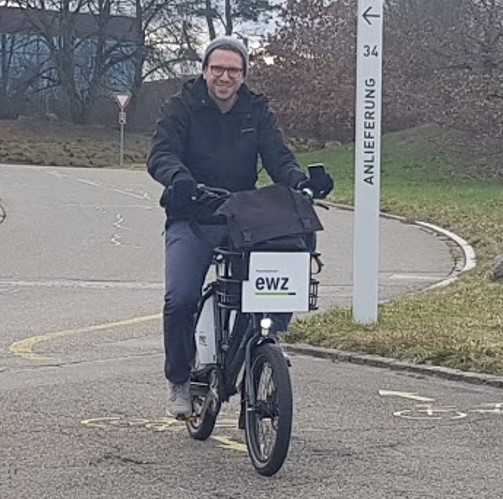
\includegraphics[width=1.0\textwidth, angle=0]{figures/Bild1.jpg}}% der eigentliche pfad mit allenfalls nötigem angle um das bild zu drehen (in grad)
{eigener schnappschuss} % die quelle (das wort quelle wird automatisch generiert)

Im code seht ihr, wie das bild eingefügt wurde. Das ist hier vom IVT so \emph{sophisticated} gemacht worden. Für latex würde eine kurze zeile reichen. Es ist dennoch sehr praktisch und mankann alles sowieso immer copypasten. So kann ich jetzt einfach auf die \cref{fig:michi} querverweisen.

Was nicht ganz so trivial ist, aber wenn mans mal drin hat super nützlich ist, ist das zitieren und einfügen von quellen. Hier mal als Beispie \citep{AxhausenEtAl_2002} oder ohne klammern \cite{AxhausenEtAl_2002}. Das codewort entnimmt man der bibliothek, welche auch hier im file ist unter \_latexfiles/bibs/all-ger.bib (habe gerade festgestellt, dass nur my.bib auf overleaf funktioniert.
Dort sind schon viele für das IVT wichtige drin abgespeichert, die man einfach kopieren kann. Wenn man was von google scholar nimmt, kann man dort auch einfach kopieren. 
Macht man jedoch einen ganz neuen eintrag wie zum beispiel vom velohandbuch, so kommt ein bisschen trial\&error zum zug... ich kann die sonst dann machen. Das braucht ein wenig übung, und selbst dann kann man durchdrehen. 

Das mühsahmste, im vergleich zu office, sind tabellen in latex. Ich kann das dann mal zeigen, wenn es soweit ist. sie sehen jedoch auch viel schöner aus am schluss:)

\cite{axhausen1909histologischen}
%%%%%%%%%%%%%%%%%%%%%%%%%%%%%%%%%%%%%%%%%%%%%%%%%%%%%%%%%%%%%%%%%%%%%%
%
\section{Analytische Anlagendimensionierung}
%
Bin jetzt dabei (Michu)!
\subsection{Resultate}
%%%%%%%%%%%%%%%%%%%%%%%%%%%%%%%%%%%%%%%%%%%%%%%%%%%%%%%%%%%%%%%%%%%%%%
hier text
\createtable[h]{Teilanlagen}{Teilanlagen}{\label{tab:reg1}}{\begin{tabular}{llllr}
\toprule
Teilanlage  &   Anlagetyp &       Nutzungsfunkt. & Wegnetz-Typologie &        Lastbild \\\midrule
Zugang Rampe Hardstr. &	Ebene Fläche&	Fortbewegung&	Zugang zur Rampe&	C \\
Rampe Hardstrasse &	Rampe &	Fortbewegung &&		C\\
Zugang Rampe Hardstr. &	Ebene Fläche&	Fortbewegung&	Kreuzungsbereich&	A,B,C\\\bottomrule
\end{tabular}}{}		

und hier

Table Generator --> google



\createtable[H]{Lastbilder}{Lastbilder}{\label{tab:reg1}}{\begin{tabular}{lrlr}
\toprule
Lastbild A &    &       Lastbild B &   \\\midrule
\specialcell{Effektive Dichte auf\\Perron $[P/m2]$} &	12421&	\specialcell{Effektive Dichte auf\\ Perron $[P/m2]$} & 325432\\
\specialcell{Zulässige Dichte auf \\Perron $[P/m2]$}&	12321&	\specialcell{Zulässige Dichte auf\\ Perron $[P/m2]$}	&2342\\\bottomrule
Lastbild C &&&\\
Treppe - Unterführung && Treppe Brücke Ost\\\midrule
\specialcell{Wirksame Länge einer\\ Türe $[m]$}&234 &&\\
\specialcell{Nutzbare Breite \\Treppe$[m]$}&234&\specialcell{Nutzbare Breite \\Treppe$[m]$}&4324\\
\specialcell{Erforderlicher\\ Abfluss $[P/s]$}&234&\specialcell{Erforderlicher \\Abfluss $[P/s]$}&234\\
\specialcell{Max. möglicher\\ Abfluss $[P/s]$}&324&\specialcell{Max. möglicher\\ Abfluss $[P/s]$}&324\\
Rückstau?&Ja&Rückstau&Nein\\
Abflussdauer$[s]$&324&Abflussdauer$[s]$&324\\\bottomrule
Lastbild D &&&\\\midrule
\specialcell{Max. spez. Fluss\\$$[P/ms]$$}& 234&\specialcell{Max. spez. Fluss\\ $$[P/ms]$$}&234\\
LOS E i. O?&ja&LOS B i.O?&nein\\\bottomrule
Lift&&&\\\midrule
Haltezeit $[s]$&324&&\\
\specialcell{Kapazität\\$[P/h/Richtung]$} &234&&\\\bottomrule
Umsteigezeit\\\midrule
Perron &234&Treppe&979\\
Strecke&234&Horizontale Strecke &234\\
\specialcell{Zeitbedarf\\Mitel}&23423&\specialcell{Zeitbedarf\\Mitel}&23423\\
\specialcell{Zeitbedarf\\Mittel – 1.5std} & 23423 &   \specialcell{Zeitbedarf\\Mittel – 1.5std}&23423\\\bottomrule
\end{tabular}}{}		

\subsection{Diskusion}

%%%%%%%%%%%%%%%%%%%%%%%%%%%%%%%%%%%%%%%%%%%%%%%%%%%%%%%%%%%%%%%%%%%%%%
%
\section{Simulation}
%
%%%%%%%%%%%%%%%%%%%%%%%%%%%%%%%%%%%%%%%%%%%%%%%%%%%%%%%%%%%%%%%%%%%%%%
\subsubsection{unter}

$i=1+1^2$

text$^2$


%%%%%%%%%%%%%%%%%%%%%%%%%%%%%%%%%%%%%%%%%%%%%%%%%%%%%%%%%%%%%%%%%%%%%%

%
%%%%%%%%%%%%%%%%%%%%%%%%%%%%%%%%%%%%%%%%%%%%%%%%%%%%%%%%%%%%%%%%%%%%%%
%%%%%%%%%%%%%%%%%%%%%%%%%%%%%%%%%%%%%%%%%%%%%%%%%%%%%%%%%%%%%%%%%%%%%%
%
\section{Schaffung von Stauräumen}
%
%%%%%%%%%%%%%%%%%%%%%%%%%%%%%%%%%%%%%%%%%%%%%%%%%%%%%%%%%%%%%%%%%%%%%%

 %\input{Section4}
%\input{Section5}
%%%%%%%%%%%%%%%%%%%%%%%%%%%%%%%%%%%%%%%%%%%%%%%%%%%%%%%%%%%%%%%%%%%%%%%
%
\section*{\ackname}%
\addcontentsline{toc}{section}{\ackname}%
%
%%%%%%%%%%%%%%%%%%%%%%%%%%%%%%%%%%%%%%%%%%%%%%%%%%%%%%%%%%%%%%%%%%%%%%

State your acknowledgements here. 
\clearpage
%%%%%%%%%%%%%%%%%%%%%%%%%%%%%%%%%%%%%%%%%%%%%%%%%%%%%%%%%%%%%%%%%%%%%%
%% Bibliography
%%   Leave this as is, and add you own entries to my.bib
%%   Many references are already defined in _latexfiles/bibs/all-eng.bib
%%   Refer to the BibTeX/LaTeX tutorial for adding new entries
%%   to the IVT BibTeX database
\bibliography{\mypath../_latexfiles/bibs/all-eng,my}
%\bibliography{_latexfiles/bibs/all-eng,my}
%%%%%%%%%%%%%%%%%%%%%%%%%%%%%%%%%%%%%%%%%%%%%%%%%%%%%%%%%%%%%%%%%%%%%%

%%%%%%%%%%%%%%%%%%%%%%%%%%%%%%%%%%%%%%%%%%%%%%%%%%%%%%%%%%%%%%%%%%%%%%
%% Appendices
%%   Usually they would start on a separate page
%%%%%%%%%%%%%%%%%%%%%%%%%%%%%%%%%%%%%%%%%%%%%%%%%%%%%%%%%%%%%%%%%%%%%%

\clearpage
%\appendix

%%%%%%%%%%%%%%%%%%%%%%%%%%%%%%%%%%%%%%%%%%%%%%%%%%%%%%%%%%%%%%%%%%%%%%
%
\section{OD-Matrix} \label{sec:a1}
%%%%%%%%%%%%%%%%%%%%%%%%%%%%%%%%%%%%%%%%%%%%%%%%%%%%%%%%%%%%%
\createtable[h]{OD-Matrix of synthetic population}{OD-Matrix of the synthetic population.}{\label{tab:odmatrix}}{\begin{tabular}{crrrrrrrrrrr}\toprule
\multicolumn{1}{l}{}                        &                         & \multicolumn{10}{c}{Destination$_j$}                                \\ 
\multicolumn{1}{l}{}                        & \multicolumn{1}{r|}{Zones}                   & 1    & 2    & 3    & 4   & 5    & 6    & 7    & 8   & 9   & 10  \\ \cline{2-12} 
\multicolumn{1}{c}{\multirow{10}{*}{\begin{turn}{90}Origin$_i$\end{turn}}} & \multicolumn{1}{r|}{1}  & 569  & 89   & 79   & 119 & 94   & 40   & 99   & 18  & 23  & 15  \\
\multicolumn{1}{c}{}                       & \multicolumn{1}{r|}{2}  & 2211 & 1283 & 762  & 550 & 857  & 505  & 419  & 151 & 145 & 138 \\
\multicolumn{1}{c}{}                       & \multicolumn{1}{r|}{3}  & 306  & 121  & 225  & 74  & 693  & 103  & 95   & 66  & 83  & 122 \\
\multicolumn{1}{c}{}                       & \multicolumn{1}{r|}{4}  & 1384 & 247  & 345  & 670 & 244  & 119  & 1296 & 157 & 84  & 111 \\
\multicolumn{1}{c}{}                       & \multicolumn{1}{r|}{5}  & 717  & 243  & 1103 & 173 & 1927 & 291  & 260  & 72  & 302 & 135 \\
\multicolumn{1}{c}{}                       & \multicolumn{1}{r|}{6}  & 1182 & 689  & 833  & 327 & 1245 & 1205 & 485  & 197 & 278 & 70  \\
\multicolumn{1}{c}{}                       & \multicolumn{1}{r|}{7}  & 842  & 132  & 159  & 763 & 268  & 124  & 1648 & 275 & 46  & 68  \\
\multicolumn{1}{c}{}                       & \multicolumn{1}{r|}{8}  & 791  & 263  & 600  & 647 & 379  & 283  & 1539 & 470 & 530 & 199 \\
\multicolumn{1}{c}{}                       & \multicolumn{1}{r|}{9}  & 265  & 55   & 180  & 85  & 789  & 114  & 55   & 114 & 99  & 15  \\
\multicolumn{1}{c}{}                       & \multicolumn{1}{r|}{10} & 221  & 111  & 565  & 229 & 375  & 45   & 165  & 96  & 26  & 341 \\ \bottomrule
\end{tabular}}{}		

\section{MNL - Biogeme output}\label{sec:mc}

\createtable[H]{MNL - Biogeme output}{MNL - Biogeme output}{\label{tab:mc}}{
 \begin{tabular}{l}
\begin{tabular}{rlr@{.}lr@{.}lr@{.}lr@{.}l}
         &                       &   \multicolumn{2}{l}{}    & \multicolumn{2}{l}{Robust}  &     \multicolumn{4}{l}{}   \\
Parameter &                       &   \multicolumn{2}{l}{Coeff.}      & \multicolumn{2}{l}{Asympt.}  &     \multicolumn{4}{l}{}   \\
number &  Description                     &   \multicolumn{2}{l}{estimate}      & \multicolumn{2}{l}{std. error}  &   \multicolumn{2}{l}{$t$-stat}  &   \multicolumn{2}{l}{$p$-value}   \\

\hline

1 & $\beta_{\text{age, bike}}$ & 0&0670 & 0&00972 & 6&89 & 0&00 \\
2 & $\beta_{\text{age, mit}}$ & -0&000180 & 0&00171 & -0&11 & 0&92 \\
3 & $\beta_{\text{age, pt}}$ & -0&00542 & 0&00214 & -2&53 & 0&01 \\
4 & $\beta_{\text{empl, bike}}$ & -0&617 & 0&255 & -2&42 & 0&02 \\
5 & $\beta_{\text{empl, mit}}$ & -1&34 & 0&172 & -7&77 & 0&00 \\
6 & $\beta_{\text{empl, pt}}$ & -0&227 & 0&118 & -1&92 & 0&05 \\
7 & $\beta_{\text{nr. o. wp, bike}}$ & -0&700 & 0&0775 & -9&03 & 0&00 \\
8 & $\beta_{\text{nr. o. wp, mit}}$ & 0&223 & 0&0388 & 5&74 & 0&00 \\
9 & $\beta_{\text{nr. o. wp, pt}}$ & 0&358 & 0&0690 & 5&19 & 0&00 \\
10 & $\beta_{\text{season, pt}}$ & 2&72 & 0&0614 & 44&34 & 0&00 \\
11 & $\beta_{\text{tt, bike}}$ & 0&0168 & 0&00506 & 3&32 & 0&00 \\
12 & $\beta_{\text{tt, mit}}$ & 0&0437 & 0&00426 & 10&27 & 0&00 \\
13 & $\beta_{\text{tt, pt}}$ & 0&0576 & 0&00451 & 12&77 & 0&00 \\
14 & $\beta_{\text{age$^2$, bike}}$ & -0&00111 & 0&000126 & -8&84 & 0&00 \\
15 & $asc_\text{bike}$ & 0&497 & 0&328 & 1&52 & 0&13 \\
16 & $asc_\text{car}$ & 1&62 & 0&205 & 7&89 & 0&00 \\
17 & $asc_\text{pt}$ & -2&62 & 0&217 & -12&05 & 0&00 \\
\hline

\end{tabular}
\\
\begin{tabular}{rcl}
\multicolumn{3}{l}{\textbf{ Summary statistics}}\\
\multicolumn{3}{l}{ Number of observations = $19798$} \\
 $\mathcal{L}(0)$ &=&  $-26993.745$ \\
 $\mathcal{L}(c)$ &=& ???\\
 $\mathcal{L}(\hat{\beta})$ &=& $-20232.034 $  \\
 $-2[\mathcal{L}(0) -\mathcal{L}(\hat{\beta})]$ &=& $13523.421$ \\
    $\rho^2$ &=&   $0.250$ \\
    $\bar{\rho}^2$ &=&    $0.250$ \\
\end{tabular}
\end{tabular}}{}		


\section{VOT - Biogeme output}\label{sec:vot}


\createtable[H]{VOT - Biogeme}{VOT - Biogeme output}{\label{tab:vot}}{
  \begin{tabular}{l}
\begin{tabular}{rlr@{.}lr@{.}lr@{.}lr@{.}l}
         &                       &   \multicolumn{2}{l}{}    & \multicolumn{2}{l}{Robust}  &     \multicolumn{4}{l}{}   \\
Parameter &                       &   \multicolumn{2}{l}{Coeff.}      & \multicolumn{2}{l}{Asympt.}  &     \multicolumn{4}{l}{}   \\
number &  Description                     &   \multicolumn{2}{l}{estimate}      & \multicolumn{2}{l}{std. error}  &   \multicolumn{2}{l}{$t$-stat}  &   \multicolumn{2}{l}{$p$-value}   \\

\hline

1 & $\beta_{\text{age, bike}}$ & -0&0276 & 0&00621 & -4&44 & 0&00 \\
2 & $\beta_{\text{age, mit}}$ & -0&00238 & 0&00152 & -1&57 & 0&12 \\
3 & $\beta_{\text{age, pt}}$ & -0&0238 & 0&00215 & -11&07 & 0&00 \\
4 & $\beta_{\text{cost, mit}}$ & -0&0391 & 0&00407 & -9&60 & 0&00 \\
5 & $\beta_{\text{dist bs, pt}}$ & -0&000383 & 6&12e-05 & -6&26 & 0&00 \\
6 & $\beta_{\text{empl, bike}}$ & 0&0571 & 0&0625 & 0&91 & 0&36 \\
7 & $\beta_{\text{empl, mit}}$ & 0&899 & 0&0531 & 16&95 & 0&00 \\
8 & $\beta_{\text{empl, pt}}$ & 1&04 & 0&0811 & 12&78 & 0&00 \\
9 & $\beta_{\text{season, pt}}$ & 2&44 & 0&0714 & 34&20 & 0&00 \\
10 & $\beta_{\text{sex, bike}}$ & -0&355 & 0&0579 & -6&12 & 0&00 \\
11 & $\beta_{\text{sex, mit}}$ & -0&755 & 0&0539 & -14&01 & 0&00 \\
12 & $\beta_{\text{sex, pt}}$ & -0&473 & 0&0771 & -6&13 & 0&00 \\
13 & $\beta_{\text{tt, bike}}$ & -0&0293 & 0&00157 & -18&69 & 0&00 \\
14 & $\beta_{\text{tt, mit}}$ & -0&0247 & 0&00446 & -5&54 & 0&00 \\
15 & $\beta_{\text{tt, pt}}$ & 0&0544 & 0&00639 & 8&51 & 0&00 \\
16 & $\beta_{\text{tt, walk}}$ & -0&00132 & 5&84e-05 & -22&59 & 0&00 \\
17 & $\beta_{\text{age$^2$, bike}}$ & 7&86e-05 & 8&09e-05 & 0&97 & 0&33 \\
18 & $asc_\text{bike}$ & 0&00876 & 0&110 & 0&08 & 0&94 \\
19 & $asc_\text{car}$ & -0&858 & 0&0800 & -10&72 & 0&00 \\
20 & $asc_\text{pt}$ & -4&10 & 0&138 & -29&76 & 0&00 \\
\hline

\end{tabular}
\\
\begin{tabular}{rcl}
\multicolumn{3}{l}{ \textbf{Summary statistics}}\\
\multicolumn{3}{l}{ Number of observations = $13985$} \\
 $\mathcal{L}(0)$ &=&  $-19314.255$ \\
 $\mathcal{L}(c)$ &=& ???\\
 $\mathcal{L}(\hat{\beta})$ &=& $-13577.733 $  \\
 $-2[\mathcal{L}(0) -\mathcal{L}(\hat{\beta})]$ &=& $11473.046$ \\
    $\rho^2$ &=&   $0.297$ \\
    $\bar{\rho}^2$ &=&    $0.296$ \\
\end{tabular}
\end{tabular}}{}		

\section{OD-Matrix for different modes}\label{seq:od_mode}

\createtable[h]{OD-Matrix by mode: walking}{OD-Matrix by mode: walking}{\label{tab:odmatrix_w}}{\begin{tabular}{crrrrrrrrrrr}\toprule
\multicolumn{1}{l}{}                        &                         & \multicolumn{10}{c}{Destination$_j$}                                \\ 
\multicolumn{1}{l}{}                        & \multicolumn{1}{r|}{Zones}                   & 1    & 2    & 3    & 4   & 5    & 6    & 7    & 8   & 9   & 10  \\ \cline{2-12} 
\multicolumn{1}{c}{\multirow{10}{*}{\begin{turn}{90}Origin$_i$\end{turn}}} & \multicolumn{1}{r|}{1}  & 113 & 18 & 16 & 24 & 19 & 8 & 20 & 3 & 4 & 3 \\ 
\multicolumn{1}{c}{}                       & \multicolumn{1}{r|}{2}  & 418 & 242 & 144 & 104 & 162 & 95 & 79 & 29 & 27 & 26 \\ 
\multicolumn{1}{c}{}                       & \multicolumn{1}{r|}{3}  &  61 & 24 & 45 & 15 & 137 & 20 & 19 & 13 & 16 & 24 \\ 
\multicolumn{1}{c}{}                       & \multicolumn{1}{r|}{4}  & 265 & 47 & 66 & 128 & 47 & 23 & 248 & 30 & 16 & 21 \\ 
\multicolumn{1}{c}{}                       & \multicolumn{1}{r|}{5}  & 135 & 46 & 207 & 32 & 362 & 55 & 49 & 14 & 57 & 25 \\ 
\multicolumn{1}{c}{}                       & \multicolumn{1}{r|}{6}  & 223 & 130 & 157 & 62 & 235 & 228 & 92 & 37 & 53 & 13 \\ 
\multicolumn{1}{c}{}                       & \multicolumn{1}{r|}{7}  & 145 & 23 & 27 & 132 & 46 & 21 & 284 & 47 & 8 & 12 \\ 
\multicolumn{1}{c}{}                       & \multicolumn{1}{r|}{8}  & 145 & 48 & 110 & 118 & 69 & 52 & 281 & 86 & 97 & 36 \\ 
\multicolumn{1}{c}{}                       & \multicolumn{1}{r|}{9}  &  50 & 10 & 34 & 16 & 148 & 21 & 10 & 21 & 19 & 3 \\ 
\multicolumn{1}{c}{}                       & \multicolumn{1}{r|}{10} & 40 & 20 & 101 & 41 & 67 & 8 & 30 & 17 & 5 & 61 \\  \bottomrule
\end{tabular}}{}


\createtable[h]{OD-Matrix by mode: cycling}{OD-Matrix by mode: cycling}{\label{tab:odmatrix_c}}{\begin{tabular}{crrrrrrrrrrr}\toprule
\multicolumn{1}{l}{}                        &                         & \multicolumn{10}{c}{Destination$_j$}                                \\ 
\multicolumn{1}{l}{}                        & \multicolumn{1}{r|}{Zones}                   & 1    & 2    & 3    & 4   & 5    & 6    & 7    & 8   & 9   & 10  \\ \cline{2-12} 
\multicolumn{1}{c}{\multirow{10}{*}{\begin{turn}{90}Origin$_i$\end{turn}}} & \multicolumn{1}{r|}{1}  & 100 & 16 & 14 & 21 & 16 & 7 & 17 & 3 & 4 & 3 \\ 
\multicolumn{1}{c}{}                       & \multicolumn{1}{r|}{2}  & 410 & 238 & 141 & 102 & 159 & 94 & 78 & 28 & 27 & 26 \\ 
\multicolumn{1}{c}{}                       & \multicolumn{1}{r|}{3}  &  59 & 23 & 43 & 14 & 133 & 20 & 18 & 13 & 16 & 23 \\ 
\multicolumn{1}{c}{}                       & \multicolumn{1}{r|}{4}  &  271 & 49 & 68 & 131 & 48 & 23 & 254 & 31 & 17 & 22 \\ 
\multicolumn{1}{c}{}                       & \multicolumn{1}{r|}{5}  &136 & 46 & 209 & 33 & 365 & 55 & 49 & 14 & 57 & 26 \\ 
\multicolumn{1}{c}{}                       & \multicolumn{1}{r|}{6}  & 216 & 126 & 152 & 60 & 227 & 220 & 89 & 36 & 51 & 13 \\ 
\multicolumn{1}{c}{}                       & \multicolumn{1}{r|}{7}  &  148 & 23 & 28 & 134 & 47 & 22 & 289 & 48 & 8 & 12 \\ 
\multicolumn{1}{c}{}                       & \multicolumn{1}{r|}{8}  &143 & 47 & 108 & 117 & 69 & 51 & 278 & 85 & 96 & 36 \\ 
\multicolumn{1}{c}{}                       & \multicolumn{1}{r|}{9}  & 51 & 11 & 34 & 16 & 151 & 22 & 11 & 22 & 19 & 3 \\ 
\multicolumn{1}{c}{}                       & \multicolumn{1}{r|}{10} &  40 & 20 & 102 & 41 & 68 & 8 & 30 & 17 & 5 & 62 \\   \bottomrule
\end{tabular}}{}


\createtable[h]{OD-Matrix by mode: public transport}{OD-Matrix by mode: public transport}{\label{tab:odmatrix_pt}}{\begin{tabular}{crrrrrrrrrrr}\toprule
\multicolumn{1}{l}{}                        &                         & \multicolumn{10}{c}{Destination$_j$}                                \\ 
\multicolumn{1}{l}{}                        & \multicolumn{1}{r|}{Zones}                   & 1    & 2    & 3    & 4   & 5    & 6    & 7    & 8   & 9   & 10  \\ \cline{2-12} 
\multicolumn{1}{c}{\multirow{10}{*}{\begin{turn}{90}Origin$_i$\end{turn}}} & \multicolumn{1}{r|}{1}  &  41 & 6 & 6 & 9 & 7 & 3 & 7 & 1 & 2 & 1 \\ 
\multicolumn{1}{c}{}                       & \multicolumn{1}{r|}{2}  & 171 & 99 & 59 & 42 & 66 & 39 & 32 & 12 & 11 & 11 \\ 
\multicolumn{1}{c}{}                       & \multicolumn{1}{r|}{3}  &  20 & 8 & 15 & 5 & 45 & 7 & 6 & 4 & 5 & 8 \\ 
\multicolumn{1}{c}{}                       & \multicolumn{1}{r|}{4}  &  97 & 17 & 24 & 47 & 17 & 8 & 91 & 11 & 6 & 8 \\ 
\multicolumn{1}{c}{}                       & \multicolumn{1}{r|}{5}  & 50 & 17 & 77 & 12 & 135 & 20 & 18 & 5 & 21 & 9 \\ 
\multicolumn{1}{c}{}                       & \multicolumn{1}{r|}{6}  & 86 & 50 & 60 & 24 & 90 & 87 & 35 & 14 & 20 & 5 \\ 
\multicolumn{1}{c}{}                       & \multicolumn{1}{r|}{7}  & 70 & 11 & 13 & 64 & 22 & 10 & 138 & 23 & 4 & 6 \\ 
\multicolumn{1}{c}{}                       & \multicolumn{1}{r|}{8}  &61 & 20 & 46 & 50 & 29 & 22 & 118 & 36 & 41 & 15 \\ 
\multicolumn{1}{c}{}                       & \multicolumn{1}{r|}{9}  & 23 & 5 & 15 & 7 & 68 & 10 & 5 & 10 & 9 & 1 \\ 
\multicolumn{1}{c}{}                       & \multicolumn{1}{r|}{10} &   16 & 8 & 42 & 17 & 28 & 3 & 12 & 7 & 2 & 25 \\   \bottomrule
\end{tabular}}{}

\createtable[h]{OD-Matrix by mode: mit}{OD-Matrix by mode: mit}{\label{tab:odmatrix_mit}}{\begin{tabular}{crrrrrrrrrrr}\toprule
\multicolumn{1}{l}{}                        &                         & \multicolumn{10}{c}{Destination$_j$}                                \\ 
\multicolumn{1}{l}{}                        & \multicolumn{1}{r|}{Zones}                   & 1    & 2    & 3    & 4   & 5    & 6    & 7    & 8   & 9   & 10  \\ \cline{2-12} 
\multicolumn{1}{c}{\multirow{10}{*}{\begin{turn}{90}Origin$_i$\end{turn}}} & \multicolumn{1}{r|}{1}  &  303 & 47 & 42 & 63 & 50 & 21 & 53 & 9 & 12 & 8 \\ 
\multicolumn{1}{c}{}                       & \multicolumn{1}{r|}{2}  & 1172 & 680 & 404 & 291 & 455 & 268 & 222 & 80 & 77 & 73 \\ 
\multicolumn{1}{c}{}                       & \multicolumn{1}{r|}{3}  &  161 & 64 & 118 & 39 & 365 & 54 & 50 & 35 & 44 & 64 \\ 
\multicolumn{1}{c}{}                       & \multicolumn{1}{r|}{4}  &  725 & 130 & 181 & 351 & 128 & 62 & 679 & 82 & 44 & 58 \\ 
\multicolumn{1}{c}{}                       & \multicolumn{1}{r|}{5}  & 383 & 130 & 589 & 92 & 1030 & 155 & 139 & 39 & 161 & 72 \\ 
\multicolumn{1}{c}{}                       & \multicolumn{1}{r|}{6}  & 635 & 370 & 448 & 176 & 670 & 648 & 261 & 106 & 149 & 38 \\ 
\multicolumn{1}{c}{}                       & \multicolumn{1}{r|}{7}  &  465 & 73 & 88 & 421 & 148 & 68 & 910 & 152 & 26 & 38 \\ 
\multicolumn{1}{c}{}                       & \multicolumn{1}{r|}{8}  &429 & 143 & 326 & 351 & 206 & 153 & 834 & 255 & 288 & 108 \\ 
\multicolumn{1}{c}{}                       & \multicolumn{1}{r|}{9}  & 136 & 28 & 93 & 44 & 407 & 59 & 28 & 59 & 51 & 8 \\ 
\multicolumn{1}{c}{}                       & \multicolumn{1}{r|}{10} & 120 & 61 & 308 & 125 & 204 & 24 & 90 & 52 & 14 & 186 \\   \bottomrule
\end{tabular}}{}





\end{document}

%%%%%%%%%%%%%%%%%%%%%%%%%%%%%%%%%%%%%%%%%%%%%%%%%%%%%%%%%%%%%%%%%%%%%%
%%%%%%%%%%%%%%%%%%%%%%%%%%%%%%%%%%%%%%%%%%%%%%%%%%%%%%%%%%%%%%%%%%%%%%
%%
%% END OF DOCUMENT
%%
%%%%%%%%%%%%%%%%%%%%%%%%%%%%%%%%%%%%%%%%%%%%%%%%%%%%%%%%%%%%%%%%%%%%%%
%%%%%%%%%%%%%%%%%%%%%%%%%%%%%%%%%%%%%%%%%%%%%%%%%%%%%%%%%%%%%%%%%%%%%%

%%%%%%%%%%%%%%%%%%%%%%%%%%%%%%%%%%%%%%%%%%%%%%%%%%%%%%%%%%%%%%%%%%%%%%
%% Editor specific keywords:
%%   This is not part of you paper, but sometimes it is used
%%   for additional features of TeX Editors.
%%
%% WinEdt:
%%   to get the bibliography list
%GATHER{./_bibs/all-eng.bib}
